\documentclass[times, utf8, zavrsni, numeric]{fer}
\usepackage{booktabs}
\usepackage{amsmath}
\usepackage{algorithm}
\usepackage{algorithmic}
\usepackage{hyperref}
% \usepackage{pdfpages}

\newcommand{\pluseq}{\mathrel{+}=}

\begin{document}

\makeatletter
\renewcommand{\ALG@name}{Algoritam}
\makeatother

% TODO: Navedite broj rada.
\thesisnumber{1160}

% TODO: Navedite naslov rada.
\title{Algoritmi za brzo učenje na neprijateljskim primjerima}

% TODO: Navedite vaše ime i prezime.
\author{Dominik Jambrović}

\maketitle

% Ispis stranice s napomenom o umetanju izvornika rada. Uklonite naredbu \izvornik ako želite izbaciti tu stranicu.
% \izvornik
% 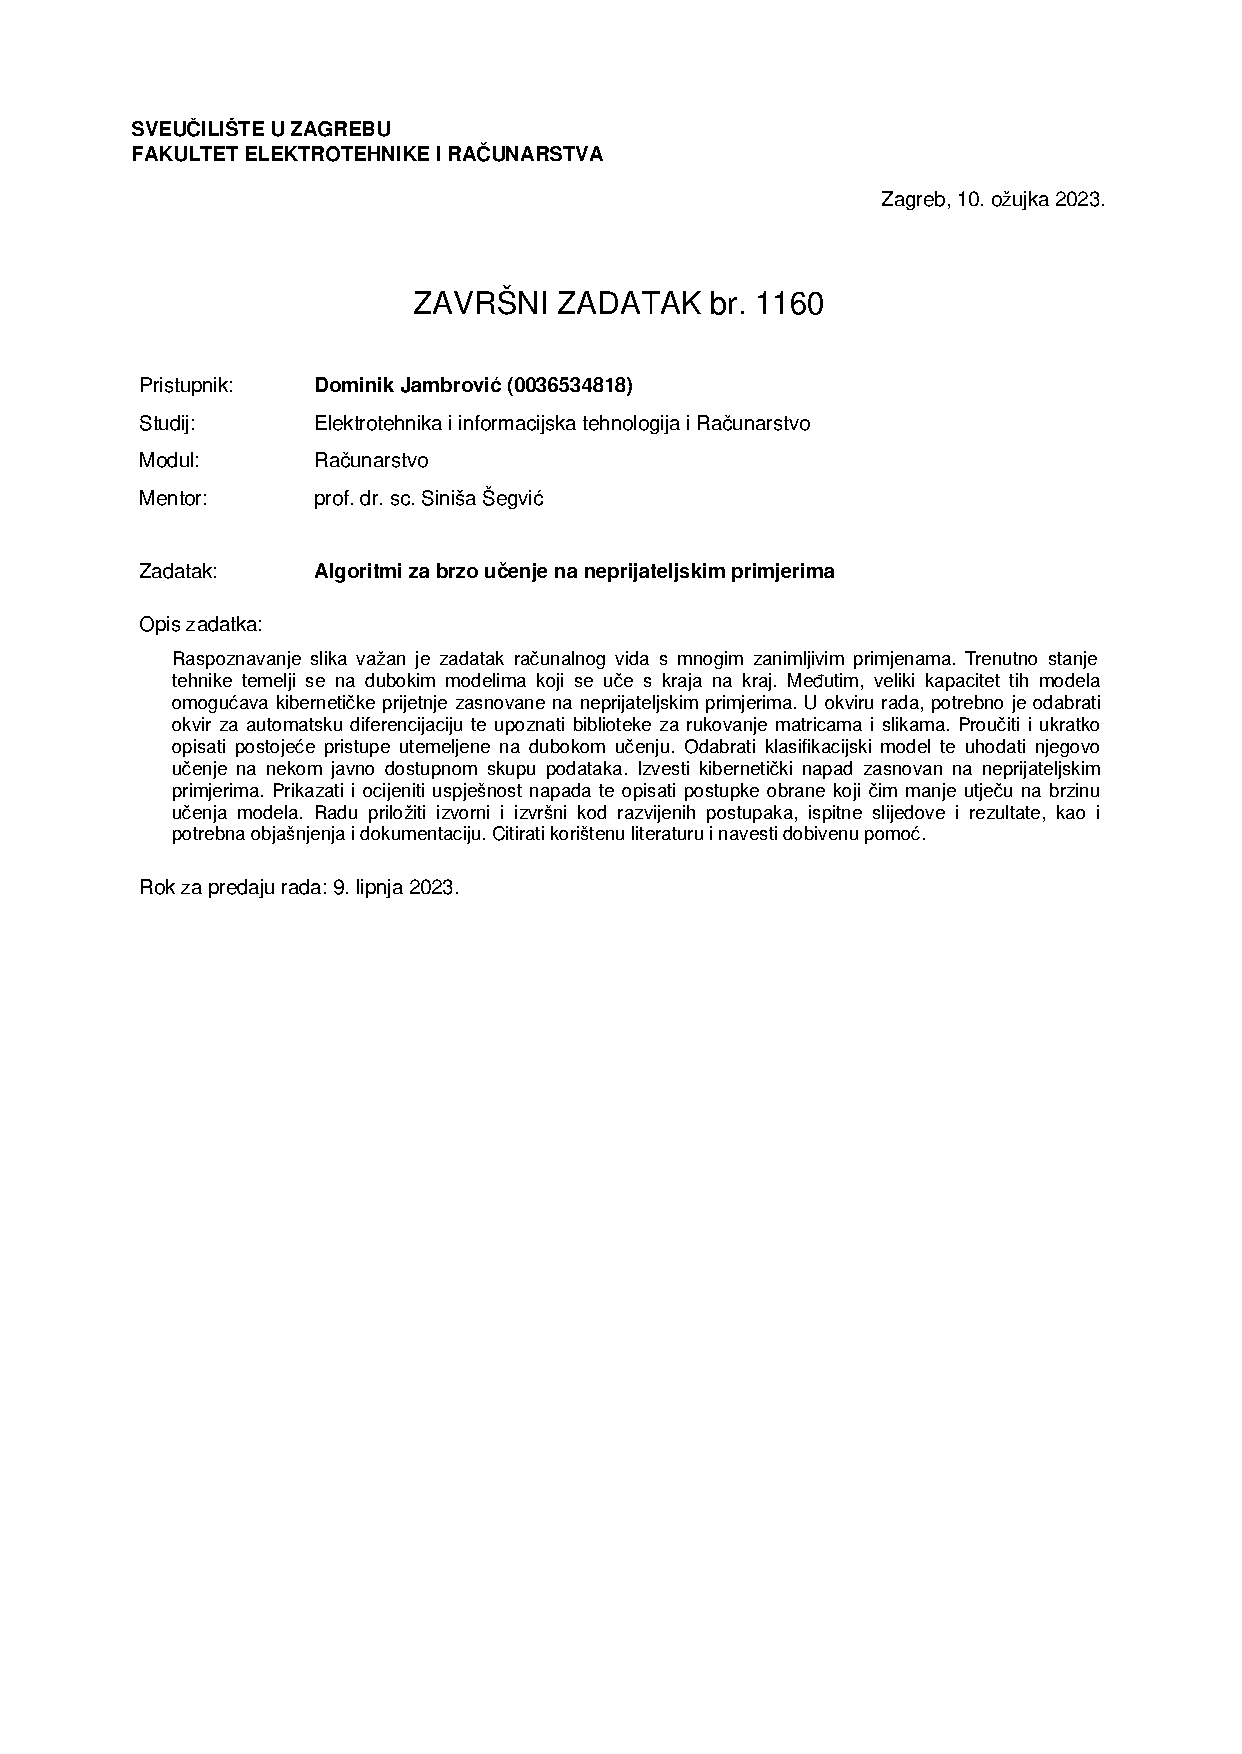
\includepdf[pages={1}]{zadatak.pdf}

\zahvala{Zahvaljujem svojoj obitelji radi podrške tijekom studiranja, kao i prof.\ dr.\ sc.\ Siniši Šegviću te mag.\ ing.\ Ivanu Grubišiću na pomoći tijekom izrade završnog rada.}

\tableofcontents

\chapter{Uvod}
Velik broj problema s kojima se danas susrećemo takve su prirode da ne znamo kako ih riješiti koristeći klasičan, algoritamski pristup. Razlog tome često leži u činjenici da ne znamo ni kako mi sami rješavamo te probleme.
Primjer jednog takvog problema je raspoznavanje tj.\ klasifikacija slika.
Trenutno najuspješniji pristupi takvim problemima temelje se na algoritmima strojnog učenja koji iskorištavaju podatke za optimiranje parametara unaprijed odabranih modela.
Pritom se kao modeli često koriste umjetne neuronske mreže - mreže sastavljene od velikog broja povezanih jedinica (neurona) koje obavljaju veoma jednostavne operacije.

Razvojem dubokih modela došlo je do ubrzanog napretka u području računalnog vida. Računalni vid područje je umjetne inteligencije koje se bavi problemima poput klasifikacije 2D slika. 
Sve većom popularizacijom i korištenjem dubokih modela u sustavima različitih namjena, u pitanje se dovodi sigurnost takvih modela -
ako model želimo koristiti u automobilima s ciljem detekcije pješaka i vozila, model mora moći dobro generalizirati, kao i biti robustan. Takav model ne bi smio mijenjati svoje odluke na temelju veoma malih promjena na ulazu.
Primjerice, htjeli bismo imati modele koji pouzdano detektiraju pješake, bez obzira nose li oni kapu ili ne.

Za ovaj rad posebno je važna robusnost na neprijateljske primjere, koja se odnosi na sposobnost modela da zadrži točnu odluku čak i u najgorem slučaju s obzirom na zadanu razinu perturbacije.
Robusnost modela možemo ostvariti različitim tehnikama. Jedna od najpopularnijih tehnika je robusno učenje tj.\ učenje na neprijateljskim primjerima. 
Kada su u pitanju modeli koji brzo uče, robusno učenje prihvatljivo je rješenje za postizanje robusnih modela otpornih na napade utemeljene na neprijateljskim primjerima. 
Ipak, kada su u pitanju veći modeli za koje učenje traje veoma dugo, standardno robusno učenje~\cite{madry2017towards} često je neprihvatljivo zbog velike računske složenosti. 
U tu svrhu, razvijene su metode koje ubrzavaju robusno učenje. U ovome radu, razmatrat ćemo tri takve metode: besplatno robusno učenje~\cite{shafahi2019adversarial}, brzo robusno učenje~\cite{wong2020fast} i
nadogradnju na brzo robusno učenje (FastAdv+ i FastAdvW,~\cite{li2020towards}). 

\pagebreak

Uz to, razmatrat ćemo i otpornost naučenih modela na zatrovane podatke. Zatrovani podatci ulazi su izmijenjeni s ciljem navođenja modela na neočekivano ponašanje. 
Uvođenjem takve ranjivosti u model, napadači mogu neprimijećeno postići proizvoljne ciljeve poput izbjegavanja detekcije ili pogrešne klasifikacije.

\chapter{Neuronske mreže}

\section{Općenito o strojnom učenju}
Strojno učenje grana je računarske znanosti čiji cilj je razvijanje algoritama koji mogu učiti na temelju podataka~\cite{uui2020ml}.
Ove algoritme možemo primjenjivati na brojne probleme. Neki od najčešćih problema su zadatci koje je teško modelirati i riješiti klasičnim algoritmima.
U ovu kategoriju spadaju problemi poput računalnog vida i raspoznavanja tj.\ klasifikacije uzoraka.
Uz ovo, algoritmi strojnog učenja često se primjenjuju i za ekstrakciju znanja iz velikih količina podataka.
Općenito govoreći, strojno učenje možemo podijeliti u tri kategorije:

\begin{enumerate}
    \item nadzirano učenje 
    \item nenadzirano učenje
    \item podržano učenje
\end{enumerate}

Kod nadziranog učenja, algoritmi na ulazu dobivaju parove oblika (ulazni podatci, očekivani izlaz). Cilj nadziranog učenja je naučiti ispravno preslikavanje ulaza na izlaz.
Kada je u pitanju nenadzirano učenje, algoritmi dobivaju samo ulazne podatke, a cilj je pronalaženje određenih pravilnosti u njima.
Podržano učenje služi za učenje optimalne strategije sustava na temelju primljenih nagrada. %Pritom sustav tj.\ agent za svoje akcije prima određenu nagradu i mijenja stanje svoje okoline, a cilj mu je maksimizirati ukupnu primljenu nagradu.
U okviru ovog rada, fokusirat ćemo se na nadzirano učenje.

Algoritam strojnog učenja sastoji se od nekoliko komponenata. Najvažnije komponente svakako su model, gubitak i optimizacijski postupak.
Pritom je model definiran parametrima koje tijekom učenja želimo poboljšavati na temelju predočenih podataka. 
Kako bi model mogao učiti, važno je definirati funkciju gubitka koja nam govori koliko su trenutni rezultati modela ispravni.
Uz ovo, veoma je važan i optimizacijski postupak kojim prilagođavamo parametre modela. 
Glavni cilj strojnog učenja je razvoj modela koji mogu dobro generalizirati tj.\ na temelju viđenih podataka zaključivati o neviđenim podatcima.

\section{Općenito o neuronskim mrežama}
Umjetne neuronske mreže veoma su popularan alat za rješavanje kompleksnih problema za koje je teško modelirati ili formalizirati znanje. 
Predstavnik su konektivističkog pristupa umjetnoj inteligenciji~\cite{uui2020} koji se zasniva na oblikovanju sustava inspiriranih građom mozga.

Problemi koje rješavamo umjetnim neuronskim mrežama većinom spadaju pod nadzirano učenje, a možemo ih svrstati u dvije glavne kategorije:
\begin{enumerate}
    \item klasifikacija 
    \item regresija
\end{enumerate}

Kada su u pitanju klasifikacijski problemi, cilj nam je svrstati ulaz u jedan od mogućih razreda. 
Pritom je na izlazu često korišteno jednojedinično kodiranje - ako ulaze svrstavamo u 10 razreda, u izlaznom sloju mreže bit će 10 neurona, a aktivacija jednog od njih predstavljat će rezultat klasifikacije.

S druge strane, kod regresijskih problema cilj nam je što bolje aproksimirati neku, modelu nepoznatu, funkciju. Za ovakve probleme, često nam je dovoljan jedan neuron u izlaznom sloju. 
Taj neuron na izlazu bi trebao davati predviđenu vrijednost funkcije za neki, do sada neviđeni, ulaz.

Da bi neuronska mreža mogla rješavati takve probleme, važno nam je da može učiti na temelju predočenih podataka. Učenje neuronske mreže odvija se izmjenom težina pojedinih neurona (time znanje implicitno ugrađujemo u našu mrežu).
Za neuronske mreže možemo reći da su algoritmi strojnog učenja kod kojih modeli tipično imaju velik broj slojeva. Pritom se kao funkcija gubitka često koristi unakrsna entropija, a kao optimizacijski postupak gradijentni spust.
Kada su u pitanju neuronske mreže s velikim brojem slojeva tj. dubinom, govorimo o pristupu strojnom učenju zvanom duboko učenje. %Za ovaj pristup potrebna nam je velika količina podataka.
Kako bismo detaljnije mogli govoriti o učenju i arhitekturama neuronskih mreža, važno je ukratko opisati neuron - osnovnu gradivnu jedinicu svake mreže.
\pagebreak
\section{Umjetni neuron}
Umjetni neuroni predstavljaju jednostavne procesne jedinice koje modeliraju ponašanje prirodnih neurona. Osnovni neuron akumulira vrijednosti na ulazu pomnožene težinama, 
akumuliranoj vrijednosti dodaje pomak te ju na kraju propušta kroz prijenosnu (aktivacijsku) funkciju. Ponašanje jednog neurona možemo modelirati jednadžbom:

\begin{equation}
    o = f(\sum_{i=1}^{n}x_{i} \cdot w_{i} + b)
    \label{eq:neuron}
\end{equation}
\\
\noindent Pritom $x$ označava pojedine ulaze, $w$ težine na pripadnim ulazima, $b$ pomak te $f$ prijenosnu funkciju. 

\section{Prijenosne funkcije}
Neki od najranijih modela umjetnog neurona kao prijenosnu funkciju koristili su funkciju identiteta (ADELINE-neuron) te funkciju skoka (TLU-perceptron).
S vremenom su korištene i razvijene brojne druge prijenosne funkcije poput sigmoidalne funkcije definirane kao:

\begin{equation}
    sigmoid(x) = \frac{1}{1 + e^{-x}}
    \label{eq:sigmoid}
\end{equation}
\\
Sigmoidalna funkcija značajna je zbog svojstva derivabilnosti nad cijelom svojom domenom. Ovo svojstvo važno je za brojne optimizacijske postupke.
Uz nju, danas je veoma značajna i zglobnica (ReLU - engl.\ \textit{Rectified Linear Unit}) koju možemo prikazati na sljedeći način:

\begin{equation}
    relu(x) = max(0, x)
    \label{eq:relu}
\end{equation}
\\
Osim navedenih prijenosnih funkcija, korištena je i softmax funkcija koju jednadžbom možemo prikazati kao:

\begin{equation}
    softmax(x_{i}) = \frac{e^{x_{i}}}{\sum_{j=1}^{n}e^{x_{j}}}
    \label{eq:softmax}
\end{equation}
\\
\pagebreak

Softmax funkcija poopćenje je sigmoidalne funkcije, a često se koristi kao zadnja prijenosna funkcija u neuronskim mrežama korištenim za klasifikaciju.
Korištenjem te funkcije u zadnjem sloju, na izlazu mreže imat ćemo vjerojatnosti klasifikacije u pojedini od razreda. Ovo svojstvo korisno nam je kada kao funkciju gubitka koristimo unakrsnu entropiju.

Važno je primijetiti da ako je prijenosna funkcija linearna, cijeli neuron može postići isključivo linearnu transformaciju. 
Kako bi umjetnim neuronima mogli modelirati kompleksnije funkcije, koristimo nelinearne prijenosne funkcije poput sigmoidalne funkcije i zglobnice. 
Pritom je za duboke neuronske mreže s velikim brojem slojeva često korištena upravo zglobnica - 
sigmoidalna funkcija za takve mreže nije prikladna zbog problema nestajućeg gradijenta (engl.\ \textit{vanishing gradient problem}) koji nastaje tijekom učenja temeljenog na gradijentnim metodama.

\section{Arhitektura umjetne neuronske mreže}
Kada je za neki problem potrebno koristiti više od jednog osnovnog neurona, neurone povezujemo u mrežu. Pritom kažemo da se neuronska mreža sastoji od nekolicine slojeva:
\begin{enumerate}
    \item ulazni sloj
    \item skriveni slojevi
    \item izlazni sloj
\end{enumerate}
Iako ulazni sloj predstavljamo neuronima, oni, za razliku od neurona u skrivenim slojevima i izlaznom sloju, ne obavljaju nikakve transformacije - možemo reći da predstavljaju ulazni podatak.
Veličina ulaznog sloja govori nam o dimenzijama ulaznih podataka, a veličina izlaznog sloja u slučaju problema klasifikacije često nam govori o broju razreda u koje klasificiramo ulaz. 

\pagebreak
\begin{figure}[htb]
    \centering
    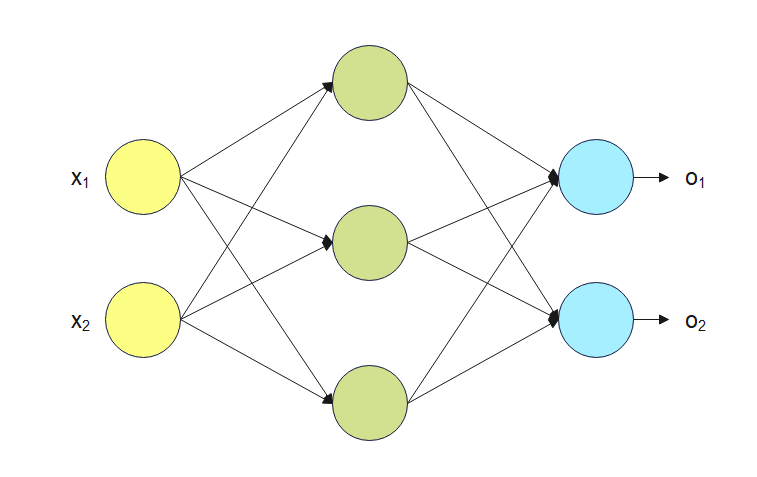
\includegraphics{basic_nn_labeled.png}
    \caption{2x3x2 arhitektura umjetne neuronske mreže.}
    \label{fig:basic_nn}
\end{figure}

Slika~\ref{fig:basic_nn} prikazuje primjer arhitekture umjetne neuronske mreže. 
Neuroni označeni žutom bojom predstavljaju ulazni sloj, neuroni označeni zelenom bojom skriveni sloj, a neuroni označeni plavom bojom izlazni sloj. 
Ovakvu arhitekturu mreže skraćeno možemo označiti kao 2x3x2 neuronsku mrežu. Pritom brojke označavaju broj neurona u pojedinom sloju (ulazni sloj je prvi sloj mreže).

Za ovakvu mrežu kažemo da je unaprijedna potpuno-povezana mreža. 
Pojam unaprijedna mreža označava to da ne postoje veze iz dubljih slojeva prema plićim slojevima, a pojam potpuno-povezana mreža označava to da svaki neuron ima vezu sa svakim neuronom iz prethodnog sloja.
Uz to, svi neuroni imaju i dodatnu težinu zvanu pomak (nije prikazano na slici~\ref{fig:basic_nn}). Djelovanje jednog sloja mreže sažeto možemo prikazati kao:

\begin{equation}
    \pmb{h}_{i} = f(\pmb{W}_{i} \cdot \pmb{h}_{i-1} + \pmb{b}_{i})
    \label{eq:nn_layer}
\end{equation}
\\
Pritom $W_{i}$ predstavlja težine trenutnog sloja, $b_{i}$ pomake trenutnog sloja, $h_{i-1}$ izlaz iz prethodnog sloja, $f$ prijenosnu funkciju primijenjenu na svaki element te $h_{i}$ izlaz iz trenutnog sloja.
Korištenjem takve formule za svaki sloj mreže, na kraju ćemo dobiti izlaz mreže za neki proizvoljni ulaz. Ovo nazivamo unaprijednim prolazom.

\section{Učenje neuronske mreže}
Kako bismo mogli koristiti proizvoljnu mrežu za probleme klasifikacije ili regresije, potrebno ju je prvo naučiti. 
Kao što je već prethodno rečeno, učenje neuronske mreže odgovara izmjeni težina pojedinih neurona, a najčešće se postiže algoritmom propagacije pogreške unatrag~\cite{Goodfellow-et-al-2016}.
Da bismo mogli znati kako trebamo izmijeniti težine neurona, prvo trebamo znati koliko naš model griješi. Mjera greške naziva se gubitak, a računa se na temelju izlaza modela i očekivanog (točnog) izlaza.
Za izračun gubitka često je korištena unakrsna entropija koju možemo definirati kao:

\begin{equation}
    H(P^{*},P) = -\sum_{i}P^{*}(i) \cdot \log{P(i)}
    \label{eq:cross_entropy}
\end{equation}
\\
Pritom $P^{*}(i)$ označava distribuciju očekivanog izlaza, a $P(i)$ distribuciju izlaza modela.
Jednom kada znamo iznos gubitka, koristeći optimizatore poput stohastičkog gradijentnog spusta (SGD) ili Adam optimizatora~\cite{kingma2014adam} možemo poboljšati naš model. 
Pritom nam je za optimizacijski postupak veoma često potreban gradijent funkcije gubitka po parametrima modela, a izračunavamo ga uzastopnom primjenom pravila ulančavanja koje u svojem najjednostavnijem obliku možemo definirati kao:

\begin{equation}
    \frac{dz}{dx} = \frac{dz}{dy} \cdot \frac{dy}{dx}
    \label{eq:chain_rule}
\end{equation}
\\
U slučaju stohastičkog gradijentnog spusta, iterativno ažuriramo težine modela na temelju iznosa gradijenta funkcije gubitka, kao i stope učenja. Sažeto postupak stohastičkog gradijentnog spusta možemo prikazati jednadžbom:

\begin{equation}
    w_{i+1} := w_{i} - \eta \cdot \nabla_{w} \cdot L(w_{i}, x)
    \label{eq:sgd}
\end{equation}
\\
Pritom $w_{i}$ označava jednu od težina modela u trenutnoj iteraciji, $w_{i+1}$ istu težinu u sljedećoj iteraciji, $L(w_{i}, x)$ funkciju gubitka, a $\eta$ stopu učenja. 
Stopa učenja mali je pozitivni broj pomoću kojeg možemo kontrolirati iznos promjene težina po iteracijama. Iterativnim ponavljanjem ovakvog postupka minimiziramo iznos funkcije gubitka, time dobivajući što bolju mrežu.
Kod stohastičkog gradijentnog spusta, iteracije mogu biti predstavljene pojedinačnim ulazima ili mini-grupama. Zbog činjenice da SGD pohranjuje gradijent za male ulaze, ovaj optimizacijski postupak zahtijeva malo memorije.

Nakon učenja mreže na skupu za učenje, evaluirat ćemo performanse mreže na neviđenom skupu zvanom skup za testiranje (engl.\ \textit{test set}). Često korištena mjera za kvalitetu modela je točnost definirana kao:

\begin{equation}
    accuracy = \frac{correct}{total}
    \label{eq:accuracy}
\end{equation}
\\
Pritom $correct$ označava broj točno klasificiranih primjera, $total$ ukupan broj primjera, a $accuracy$ točnost.
Uz točnost, postoje i brojne druge mjere kvalitete modela. Neke od njih su preciznost (engl.\ \textit{precision}), odziv (engl.\ \textit{recall}) i matrica zabune (engl.\ \textit{confusion matrix}).

\section{Duboke neuronske mreže}
Ako želimo rješavati složenije probleme koristeći umjetne neuronske mreže sa samo jednim skrivenim slojem, suočit ćemo se s problemom - broj neurona potreban kako bi umjetna neuronska mreža mogla obavljati svoju zadaću bit će prevelik.
Uz to, korištenjem širokog modela s velikim brojem neurona u skrivenom sloju teško ćemo postići svojstvo generalizacije jer će se model lako prenaučiti i zapamtiti ulazne podatke. 

Zbog tih razloga, veoma su popularne duboke neuronske mreže~\cite{Goodfellow-et-al-2016}. Duboke neuronske mreže, za razliku od mreža sa samo jednim skrivenim slojem, imaju nekolicinu skrivenih slojeva. 
Pritom za rješavanje složenijih problema duboke mreže trebaju imati značajno manje neurona po sloju naspram mreže sa samo jednim skrivenim slojem. 
Zasebni slojevi mreže naučit će prepoznavati zasebne značajke ulaza, a njihovom kombinacijom mreža će moći postići uspješnu klasifikaciju.

Ipak, postoje i određene mane dubokih neuronskih mreža. Jedna od mana činjenica je da je za propagaciju pogreške unazad kod ovakvih mreža potrebno množiti gradijente. 
U slučaju da kao prijenosnu funkciju koristimo sigmoidalnu funkciju, ovo lako vodi do problema nestajućeg gradijenata zbog kojega težine neurona u plitkim slojevima nećemo moći ispravno izmijeniti.
Uz problem nestajućeg gradijenta, postoji i problem eksplodirajućeg gradijenta (engl.\ \textit{exploding gradient problem}) koji se pojavljuje kod nekih drugih prijenosnih funkcija od kojih je najpoznatija upravo zglobnica (ReLU).
Još jedna mana dubokih neuronskih mreža činjenica je da kako bismo kvalitetno naučili duboku mrežu moramo imati veoma velik skup podataka.

\section{Konvolucijske mreže}
Za probleme s velikim dimenzijama ulaza, potpuno-povezane mreže imaju izuzetno velik broj parametara tj.\ težina neurona. 
Učenje ovakvih modela zahtijeva veliku količinu memorije, a i općenito je sporo. 
Uz to, potpuno-povezane mreže osjetljive su na translaciju ulaza: ako učimo mrežu da klasificira slike vozila te nakon učenja mreži predočimo translatiranu sliku iz skupa za učenje, mreža tu sliku neće nužno moći ispravno klasificirati jer je za nju to potpuno novi podatak.
Ovo svojstvo proizlazi iz činjenice da je svaki neuron ovisan o svakom neuronu iz prethodnog sloja.

Kako bi doskočili ovim problemima, uvedene su konvolucijske mreže~\cite{o2015introduction}. 
Za razliku od potpuno-povezanih mreža, ovdje aktivacija neurona ne ovisi o svim neuronima iz prethodnog sloja, već samo o malom rasponu neurona iz prethodnog sloja. 
Time konvolucijska mreža ima značajno manje parametara naspram potpuno-povezane mreže iste dubine, a postiže i svojstvo translacijske invarijantnosti.
Ova svojstva konvolucijska mreža postiže zamjenom standardnog množenja matrica operacijom konvolucije s jezgrom (engl.\ \textit{kernel}). 
Općenito govoreći, operaciju konvolucije za dvije funkcije $f, g$ možemo definirati kao:

\begin{equation}
    (f * g)(t) := \int_{-\infty}^{\infty}f(\tau) \cdot g(t-\tau)d\tau
    \label{eq:convolution}
\end{equation}
\\
Operacija konvolucije opisuje nam kako se izgled jedne funkcije mijenja pod utjecajem druge funkcije, 
a definirana je kao integral umnoška funkcija nakon što je jedna reflektirana i translatirana. 
Uz operaciju konvolucije postoji i unakrsna korelacija definirana kao:

\begin{equation}
    (f \star g)(t) := \int_{-\infty}^{\infty}f(\tau) \cdot g(t+\tau)d\tau
    \label{eq:correlation}
\end{equation}
\\
Važno je primijetiti da je glavna razlika između te dvije operacije izostajanje reflektiranja jedne od funkcija u slučaju operacije unakrsne korelacije. 
Kada kod konvolucijskih mreža govorimo o konvoluciji, gotovo uvijek se zapravo misli na unakrsnu korelaciju.

Kako bismo što jednostavnije objasnili konvoluciju, koristit ćemo primjer s 2D konvolucijom.
U tom slučaju, jezgra s kojom se provodi konvolucija mala je kvadratna matrica s težinama koje učenjem izmjenjujemo. Skalarnim produktom dijelova ulazne matrice i jezgre dobivamo izlaz konvolucijskog sloja.
Pritom se jezgra pomiče po ulaznoj matrici, a rezultati skalarnog produkta zapisuju se u novu matricu koju zovemo mapa značajki.

\pagebreak
\begin{figure}[htb]
    \centering
    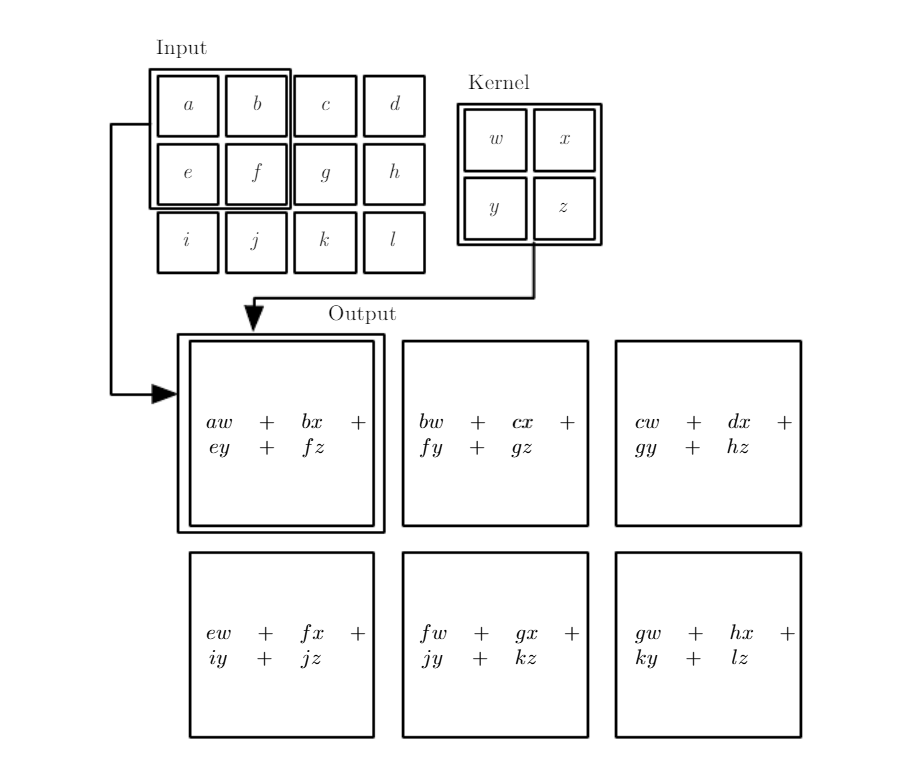
\includegraphics[scale=0.5]{convolution.png}
    \caption{Primjer 2D konvolucije. Preuzeto iz~\cite{Goodfellow-et-al-2016}.}
    \label{fig:convolution}
\end{figure}

Slika~\ref{fig:convolution} prikazuje rezultat 2D konvolucije s ulaznom matricom veličine 3x4 i jezgrom dimenzija 2x2. 
Mapa značajki nastala kao rezultat ove konvolucije dimenzija je 2x3. Primijetimo da će izlaz konvolucijskog sloja uvijek biti manjih dimenzija naspram ulaza.
Uz to, vrijednosti na rubovima matrice ulaza manje će doprinijeti rezultatu naspram vrijednosti koje su dalje od rubova.

Kako bismo imali veću kontrolu nad dimenzijama izlaza, kao i utjecajem vrijednosti na rubovima matrice ulaza, često koristimo nadopunjavanje nulama (engl.\ \textit{zero padding}).

\begin{figure}[htb]
    \centering
    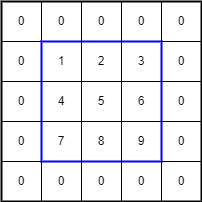
\includegraphics[scale=0.5]{zero_padding.png}
    \caption{Primjer nadopunjavanja 3x3 matrice nulama.}
    \label{fig:zero_padding}
\end{figure}

Slika~\ref{fig:zero_padding} prikazuje 3x3 matricu nadopunjenu nulama. U slučaju da nad takvom matricom primijenimo konvoluciju s jezgrom dimenzija 2x2, mapa značajki na izlazu bila bi dimenzija 4x4.
Da smo konvoluciju primijenili nad matricom bez nadopunjavanja, mapa značajki bila bi dimenzija 2x2, a vrijednosti pri rubovima matrice manje bi joj doprinosile.
Možemo reći da nule čine okvir oko originalne matrice, time osiguravajući veće dimenzije izlaza.

\pagebreak

Uz nadopunjavanje nulama, kod konvolucijskih slojeva često se mijenja i korak (engl.\ \textit{stride}). 
Na slici~\ref{fig:convolution} korak je 1, a definira za koliko se ćelija horizontalno i vertikalno pomiče jezgra. 
U slučaju da povećamo korak, izlaz konvolucije bio bi manjih dimenzija, a time bi se i ubrzao postupak računanja izlaza.
\begin{figure}[htb]
    \centering
    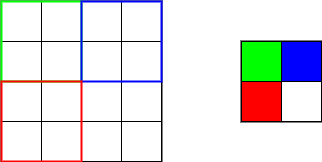
\includegraphics[scale=0.5]{stride.png}
    \caption{Primjer konvolucije s korakom 2.}
    \label{fig:stride}
\end{figure}

Slika~\ref{fig:stride} prikazuje konvoluciju s korakom 2. Za razliku od standardnog kretanja jezgre, ovdje se jezgra nakon svakog izračuna pomiče za 2 ćelije. 

Osim samih konvolucijskih slojeva, konvolucijske mreže u sebi sadrže i slojeve sažimanja. 
Najčešći razlog za upotrebu slojeva sažimanja je smanjivanje dimenzija podataka, a time i skraćivanje vremena potrebnog za učenje mreže.

\begin{figure}[htb]
    \centering
    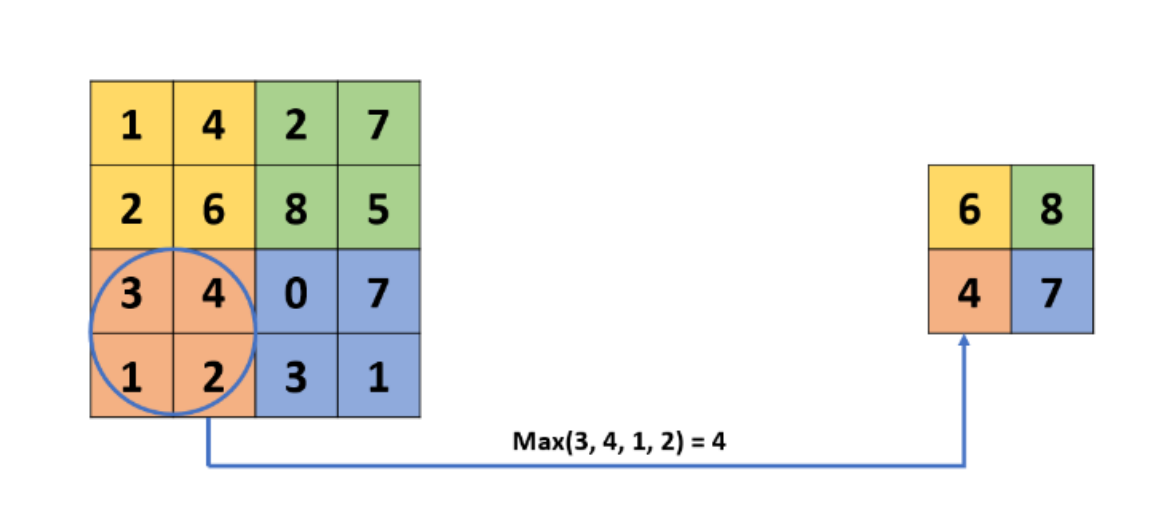
\includegraphics[scale=0.35]{maxpool.png}
    \caption{Primjer sažimanja maksimalnom vrijednošću. Preuzeto iz~\cite{gholamalinezhad2020pooling}.}
    \label{fig:maxpool}
\end{figure}

Slika~\ref{fig:maxpool} prikazuje primjer korištenja sloja sažimanja maksimalnom vrijednošću.
Mapa značajki dimenzija 4x4 korištenjem sažimanja maksimalnom vrijednošću 2x2 (engl.\ \textit{2x2 max pooling}) smanjena je na dimenzije 2x2, efektivno smanjujući dimenzije ulaza za faktor 2.
Uz sažimanje maksimalnom vrijednošću, veoma je popularno i sažimanje usrednjavanjem, no postoje i brojne druge varijante koje se koriste za slojeve sažimanja.
Kao i operacija konvolucije, i slojevi sažimanja doprinose translacijskoj invarijantnosti, osiguravajući da mreža lako može prepoznati neku značajku bez obzira na njenu točnu lokaciju.

\section{Rezidualne mreže}

Rezidualne mreže~\cite{he2016deep} vrsta su dubokih neuronskih mreža koje koriste rezidualne blokove. Općenito govoreći, blok u kontekstu neuronskih mreža označava niz od nekoliko slojeva. 
Pojedini blokovi mogu se kombinirati kako bi sačinjavali složeniju mrežu. 
Rezidualni blokovi najčešće se sastoje od nekoliko konvolucijskih slojeva, a njihova glavna karakteristika postojanje je preskočnih veza.

\begin{figure}[htb]
    \centering
    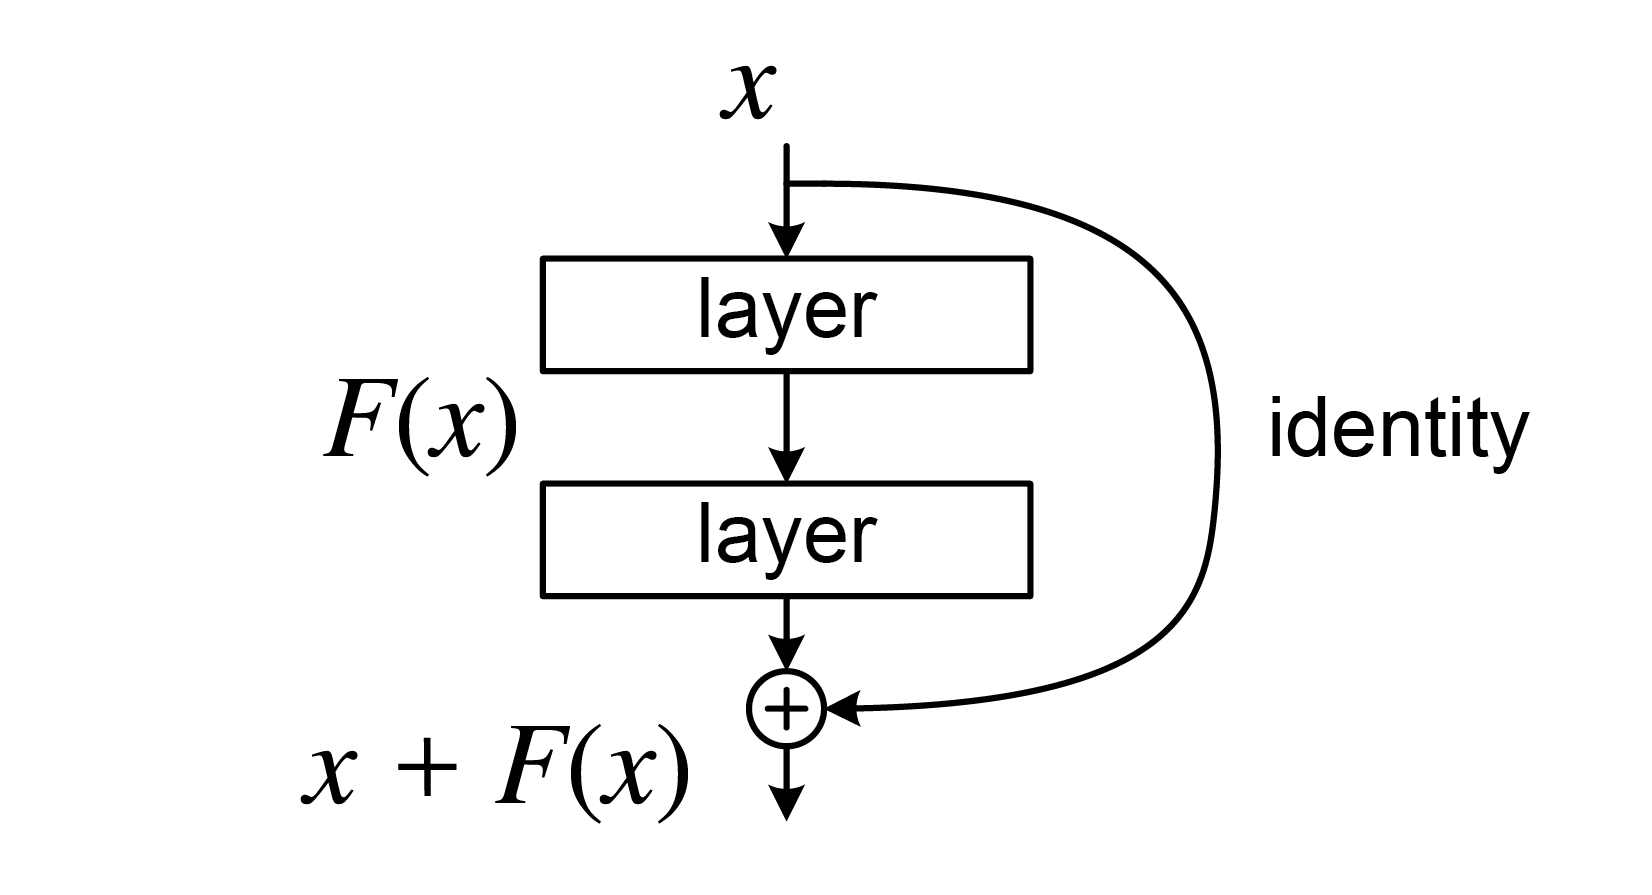
\includegraphics{ResBlock.png}
    \caption{Primjer rezidualnog bloka. Preuzeto iz~\cite{he2016deep}.}
    \label{fig:resblock}
\end{figure}

Slika~\ref{fig:resblock} prikazuje rezidualni blok sačinjen od dva sloja. Preskočna veza ulaz u blok bez ikakvih transformacija prenosi na izlaz. 
Ovakvim strukturiranjem mreže, cilj mreže postaje modelirati rezidualnu funkciju $F(x)$ koja mjeri razliku izlaza naspram ulaza. Rezidualni blok možemo prikazati jednadžbom:

\begin{equation}
    f(\pmb{x}) = F(\pmb{x}) + \pmb{x}
    \label{eq:resblock}
\end{equation}
\\
Pritom $F(x)$ predstavlja rezidualnu funkciju, $x$ prenošenje ulaza na izlaz preskočnom vezom, a $f(x)$ izlaz bloka. 
U slučaju da slojevi između mijenjaju dimenzije podataka, preskočna veza morat će raditi linearnu projekciju kako bi podatci pri zbrajanju bili istih dimenzija. 
Tada rezidualni blok možemo prikazati na sljedeći način:

\begin{equation}
    f(\pmb{x}) = F(\pmb{x}) + \pmb{W}_{s} \cdot \pmb{x}
    \label{eq:resblocklp}
\end{equation}
\\
Pritom $W_{s}$ označava matricu korištenu za linearnu projekciju ulaza $x$. 
Korištenje slojeva s preskočnim vezama motivirano je željom za učenjem funkcije identiteta.
Klasične duboke mreže s velikim brojem slojeva teško će naučiti funkciju identiteta, dok korištenje preskočnih veza dubokim mrežama značajno olakšava učenje te funkcije.
Ovo potječe od činjenice da je za uspješno modeliranje funkcije identiteta $f(x)$ za rezidualnu funkciju $F(x)$ potrebno samo postaviti težine jezgri na 0.

\section{ResNet-18}

U okviru ovog rada, za provođenje svih eksperimenata koristit ćemo ResNet-18 mrežu kako bismo što bolje mogli usporediti učinak različitih eksperimenata. 
ResNet-18 rezidualna je neuronska mreža, a sastoji se od ukupno 18 slojeva. 

\begin{figure}[htb]
    \centering
    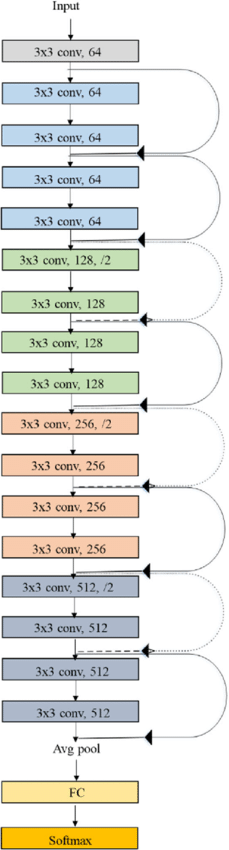
\includegraphics[scale=0.7]{resnet18.png}
    \caption{Arhitektura ResNet-18. Preuzeto iz~\cite{mcc19}.}
    \label{fig:resnet-18}
\end{figure}

Kao što možemo vidjeti na slici~\ref{fig:resnet-18}, ResNet-18 sastoji se od 8 rezidualnih blokova. Svaki od tih blokova sastoji se od 2 konvolucijska sloja i jedne preskočne veze.
Rezidualnim blokovima prethodi jedan konvolucijski sloj, a nakon njih dolazi jedan potpuno-povezani sloj sa softmax prijenosnom (aktivacijskom) funkcijom.

\chapter{Brzo učenje na neprijateljskim primjerima}

\section{Neprijateljski primjeri}

Kada učimo modele da rješavaju razne probleme, cilj nam je da modeli pokažu svojstvo generalizacije. 
U slučaju problema klasifikacije, to znači da bi modeli trebali dobro klasificirati i do sada neviđene primjere.
Mogućnost generalizacije određenog modela najčešće provjeravamo koristeći unakrsnu provjeru (engl.\ \textit{cross-validation}).
Pritom skup podataka dijelimo na 2 ili 3 skupa: 

\begin{enumerate}
    \item skup za učenje (engl.\ \textit{train set})
    \item skup za provjeru (engl.\ \textit{validation set})
    \item skup za testiranje (engl.\ \textit{test set})
\end{enumerate}

Skup za učenje modelu predočavamo kako bi na temelju njega mogao poboljšavati svoje parametre tj.\ učiti. 
S druge strane, skup za provjeru koristimo za poboljšavanje hiperparametara modela (npr.\ stopa učenja modela). 
U slučaju da smo sigurni u dobar odabir hiperparametara modela, korištenje ovog skupa nije nužno. 
Nakon postupka učenja, koristeći skup za testiranje evaluiramo model kako bismo dobili procjenu njegove generalizacijske pogreške.

Općenito govoreći, model će na skupu za testiranje postizati lošije rezultate naspram rezultata na skupu za učenje. 
Ako model dobro generalizira, razlika između rezultata na ta dva skupa neće biti veoma značajna. 
Ipak, u zadnjih desetak godina otkriveni su načini za konstrukciju ulaznih slika koje će zadani model vrlo loše klasificirati iako na većini prirodnih slika dobro generalizira. 
Takve ulaze zvat ćemo neprijateljski primjeri~\cite{goodfellow2014explaining}.

\pagebreak

\begin{figure}[htb]
    \centering
    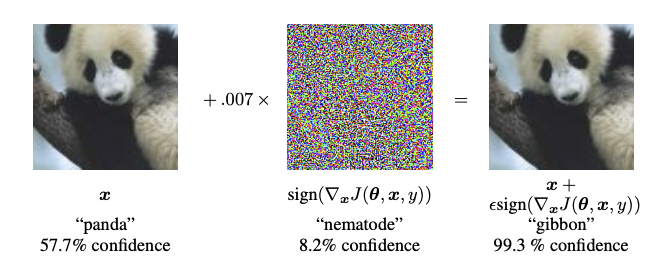
\includegraphics[scale=0.5]{adversarial_example.png}
    \caption{Primjer neprijateljskog primjera. Preuzeto iz~\cite{goodfellow2014explaining}.}
    \label{fig:adv_example}
\end{figure}

Slika~\ref{fig:adv_example} prikazuje jedan neprijateljski primjer.
Originalni ulaz kojeg model ispravno klasificira izmijenjen je za iznos perturbacije.
U ovom slučaju iznos perturbacije dobiven je kao umnožak malog pozitivnog koeficijenta $\epsilon$ i predznaka gradijenta gubitka po ulazu.
Iako je izmijenjeni ulaz ljudima gotovo identičan, model ovaj ulaz krivo klasificira, a pritom je veoma siguran u svoju odluku.
Ovo svojstvo iskazali su brojni modeli te je zbog toga u zadnjih desetak godina porastao interes za proučavanjem neprijateljskih primjera.

\section{Konstrukcija neprijateljskih primjera}

Neprijateljske primjere moguće je konstruirati na različite načine. 
Načine konstrukcije neprijateljskih primjera zovemo napadima, a možemo ih podijeliti na usmjerene i neusmjerene napade.
Usmjereni napadi kao cilj imaju konstrukciju neprijateljskih primjera koje će napadnuti model klasificirati u točno jedan ciljni razred,
dok neusmjereni napadi kao cilj imaju konstrukciju neprijateljskih primjera koje će napadnuti model što lošije klasificirati, neovisno o konkretnom razredu.
Pronalaženje neprijateljskih primjera zapravo je optimizacijski problem koji možemo prikazati sljedećim izrazom:

\begin{equation}
    \underset{\delta \in [-\epsilon, \epsilon]}{max}L(x + \delta,y;\theta)
    \label{eq:adversarial_optimization}
\end{equation}
\\
Pritom $\delta$ označava iznos perturbacije u intervalu određenim s granicama $[-\epsilon, \epsilon]$, $L(x,y;\theta)$ funkciju gubitka, a $\theta$ parametre modela.
Drugim riječima, cilj nam je naći perturbaciju omeđenu određenim iznosom takvu da je iznos funkcije gubitka za ulaz izmijenjen tom perturbacijom maksimalan.
Iznos perturbacije najčešće je omeđen L\textsubscript{$\infty$} normom, no može biti omeđen i L\textsubscript{2} normom ili L\textsubscript{1} normom. 

U slučaju vektorskog prostora, L\textsubscript{$\infty$} norma bit će jednaka iznosu najveće apsolutne vrijednosti komponente vektora, L\textsubscript{2} norma euklidskoj udaljenosti vektora od ishodišta, a L\textsubscript{1} norma sumi iznosa apsolutnih vrijednosti svih komponenti vektora.
Općenito govoreći, L\textsubscript{p} normu možemo definirati sljedećom formulom:

\begin{equation}
    \lVert x \rVert_{p} = \sqrt[p]{\sum_{i = 1}^{n}|x_{i}|^p}
    \label{eq:lpnorm}
\end{equation}
\\
Formula~\ref{eq:lpnorm} vrijedi za proizvoljan broj $p$ veći od 0. Ipak, L\textsubscript{$\infty$} normu uobičajeno definiramo zasebnom formulom:

\begin{equation}
    \lVert x \rVert_{\infty} = \max_{i}(|x_{i}|)
    \label{eq:linfnorm}
\end{equation}
\\
Postoje brojni načini konstrukcije neprijateljskih primjera. 
Neki od najpoznatijih napada poznati su pod nazivima FGSM (engl.\ \textit{Fast Gradient Sign Method})~\cite{goodfellow2014explaining} i PGD (engl.\ \textit{Projected Gradient Descent})~\cite{madry2017towards} napadi.
Primjer sa slike~\ref{fig:adv_example} zapravo je neprijateljski primjer konstruiran napadom FGSM, a tako dobivene neprijateljske primjere sažeto možemo opisati jednadžbom:

\begin{equation}
    x_{adv} := x + \epsilon \cdot sign(\nabla_{x}L(x,y;\theta))
    \label{eq:fgsm}
\end{equation}
\\
Pritom $\epsilon$ predstavlja mali pozitivan broj koji određuje veličinu perturbacije, $x$ ulazni podatak, $sign(x)$ predznak od $x$, a $x_{adv}$ konstruirani neprijateljski primjer. 
Napad FGSM originalnom ulazu pridodaje iznos istog predznaka kao i gradijent funkcije gubitka. Time se osigurava najveći mogući rast iznosa funkcije gubitka. 
Ovakav napad primjer je neusmjerenog napada. U slučaju usmjerenog napada, cilj bi nam bio što više smanjiti iznos funkcije gubitka s obzirom na proizvoljan razred.

Uz napad FGSM, postoji i napad koji iterativno stvara značajno učinkovitije neprijateljske primjere. 
Tu vrstu napada zovemo napad PGD (projicirani gradijentni spust). Za razliku od FGSM-a, napad PGD iterativno ponavlja postupak, time postižući gradijentni spust.
Na kraju svake iteracije, trenutna perturbacija projicira se na L\textsubscript{p} loptu definiranu unaprijed zadanim koeficijentom $\epsilon$.
Ovim postupkom pokušavamo odrediti najbolje rješenje optimizacijskog problema~\ref{eq:adversarial_optimization}.

\begin{algorithm}
    \caption{Konstrukcija neprijateljskih primjera napadom PGD}
    \label{algo:pgd}
    \begin{algorithmic}
        \STATE{\textbf{Ulaz:} $x$ -- ulazne slike, $y$ -- ispravne oznake ulaznih slika, $\epsilon$ -- ograničenje perturbacije, $\alpha$ -- veličina koraka po iteraciji, $K$ -- broj iteracija za konstrukciju neprijateljskih primjera}
        \STATE{\textbf{Izlaz:} $x_{adv}$ -- neprijateljski primjeri konstruirani napadom PGD}
        \\\hrulefill
        \STATE{$\delta = U(-\epsilon, \epsilon)$}
        \FOR{($i = 1 \dots K$)}
            \STATE{$grad = \nabla_{\delta}L(x + \delta,y;\theta)$}
            \STATE{$\delta = \delta + \alpha \cdot sign(g)$}
            \STATE{$\delta = clamp(\delta, -\epsilon, \epsilon)$}
        \ENDFOR
        \STATE{$x_{adv} = x + \delta$}
        \RETURN{$x_{adv}$}
    \end{algorithmic}
\end{algorithm}

\pagebreak

Pseudokod~\ref{algo:pgd} prikazuje način konstrukcije neprijateljskih primjera PGD-om. 
Perturbacija $\delta$ na početku je inicijalizirana pomoću uniformne distribucije s rasponom $[-\epsilon, \epsilon]$, 
a na kraju svake iteracije iznos perturbacije ograničava se koristeći funkciju \textit{clamp} kojom postižemo projiciranje na L\textsubscript{$\infty$} loptu. 
Naravno, postoje brojni načini inicijalizacije iznosa perturbacije, no nasumična inicijalizacija pokazala se dosta uspješnom.
Važno je istaknuti da pseudokod za ograničavanje iznosa perturbacije koristi L\textsubscript{$\infty$} normu. 
Napad PGD s $K$ iteracija za konstrukciju neprijateljskih primjera zvat ćemo K-PGD (npr.\ 20-PGD).

\section{Učenje na neprijateljskim primjerima}

Ako želimo da modeli koje učimo budu otporni na neprijateljske primjere tj.\ ispravno ih klasificiraju, ne možemo se ograničiti na klasično (prirodno) učenje modela.
Kao što je već rečeno, svojstvo otpornosti na neprijateljske primjere zvat ćemo robusnost iako se u literaturi ovaj naziv zna koristiti i u drugim kontekstima.
Jedan od mogućih načina za postizanje robusnih modela učenje je na neprijateljskim primjerima (robusno učenje).
Kada govorimo o robusnom učenju, općenita ideja je da se tijekom učenja konstruiraju neprijateljski primjeri prilagođeni samome modelu.
Model tada ne uči na originalnim ulaznim podatcima, već isključivo na konstruiranim neprijateljskim primjerima.
U tom slučaju neprijateljske primjere možemo smatrati načinom augmentacije ulaznih podataka. % - na temelju originalnih ulaznih podataka stvaramo nove podatke koje predočavamo modelu.

\pagebreak

Robusnim učenjem možemo postići puno višu točnost modela na skupu za testiranje sačinjenom od neprijateljskih primjera naspram modela učenih prirodnim učenjem.
Nažalost, robusno učenje ima svoju cijenu. Robusni modeli gotovo uvijek će na originalnom skupu za testiranje imati nižu točnost naspram modela učenih prirodnim učenjem,
a i učit će se dulje. Ako za konstrukciju neprijateljskih primjera tijekom robusnog učenja koristimo metodu FGSM, učenje će trajati otprilike dvostruko dulje naspram prirodnog učenja
jer je za konstrukciju neprijateljskih primjera metodom FGSM potreban dodatan unaprijedni prolaz kroz mrežu. 
Ako za konstrukciju neprijateljskih primjera koristimo metodu PGD, duljina trajanja učenja ovisit će o broju iteracija korištenih za konstrukciju neprijateljskih primjera.
Koristimo li 10 iteracija za konstrukciju neprijateljskih primjera, učenje će trajati otprilike 11 puta dulje naspram prirodnog učenja. 
Općenito govoreći, kako bismo model učili K-PGD-om, učenje će trajati otprilike K + 1 puta dulje naspram prirodnog učenja~\cite{shafahi2019adversarial}.

\begin{algorithm}
    \caption{Učenje na neprijateljskim primjerima}
    \label{algo:adv_learning}
    \begin{algorithmic}
        \STATE{\textbf{Ulaz:} $x$ -- ulazne slike, $y$ -- ispravne oznake ulaznih slika, $N$ -- broj epoha, $M$ -- veličina skupa za učenje, $K$ -- broj iteracija za konstrukciju neprijateljskih primjera, $\eta$ -- stopa učenja, $\epsilon$ -- ograničenje perturbacije, $\alpha$ -- veličina koraka po iteraciji}
        \\\hrulefill
        \STATE{$\theta = initializeModelParams()$}
        \FOR{$(ep = 1 \dots N)$}
            \STATE{$grad = 0$}
            \FOR{$(i = 1 \dots M)$}
                \STATE{$x_{adv} = generateAdversarial(x_{i}, y_{i}, \epsilon, \alpha, K)$}
                \STATE{$grad \pluseq \nabla_{\theta}L(x_{adv},y_{i};\theta)$}
            \ENDFOR
            \STATE{$\theta = \theta - \eta \cdot grad$}
        \ENDFOR
    \end{algorithmic}
\end{algorithm}

Pseudokod~\ref{algo:adv_learning} prikazuje općeniti algoritam za učenje na neprijateljskim primjerima.
Pritom inicijalizaciju parametara modela $\theta$ prikazujemo pozivom funkcije \textit{initializeModelParams}.
Radi općenitosti, konstrukcija neprijateljskih primjera prikazana je pozivom funkcije \textit{generateAdversarial}.
% Ta funkcija mogla bi konstruirati neprijateljske primjere koristeći FGSM metodu, PGD metodu ili neki alternativan način, no to nam za općeniti prikaz nije važno.
Bitno je istaknuti da se u konkretnim implementacijama funkcija \textit{generateAdversarial} koristi za konstruiranje neprijateljskih primjera na temelju mini-grupe.
U tom slučaju, i izračun gradijenta primjenjuje se na cijelu mini-grupu.

\section{Brzo učenje na neprijateljskim primjerima}

U slučaju da model koji učimo nije veoma složen, obično učenje na neprijateljskim primjerima prihvatljiv je način za postizanje robusnih modela otpornih na napade.
Ipak, ako učimo složene modele na velikim skupovima podataka, obično učenje na neprijateljskim primjerima presporo je. 
Uz to, rijetko tko uopće posjeduje dovoljnu količinu računalnih resursa za robusno učenje složenijih modela.
Kako bismo riješili ili barem umanjili ovaj problem, predložena su brojna rješenja čijom bi se primjenom ubrzalo robusno učenje. Razmotrit ćemo tri takva rješenja.

\subsection{"Besplatno" učenje na neprijateljskim primjerima}

Jedno od prvih predloženih rješenja za problem duljine trajanja učenja robusnih modela naziva se "besplatno" učenje (engl.\ \textit{free adversarial training})~\cite{shafahi2019adversarial}.
Uočeno je da modeli učeni PGD-om imaju visoku robusnost, no, kao što je već rečeno, zahtijevaju puno vremena za učenje.

Osnovna ideja "besplatnog" učenja je sljedeća: unatražnim prolazom izračunamo gradijent po ulazu potreban za konstrukciju neprijateljskih primjera, kao i gradijent po parametrima modela.
Kako bismo iterativno konstruirali što kvalitetnije neprijateljske primjere, tijekom učenja modelu na ulaz nekoliko puta dovodimo istu mini-grupu prije nego što pređemo na sljedeću.
Ponavljanjem mini-grupe nekoliko puta zaredom pokušavamo postići postupak sličan PGD-u, a da pritom ne platimo veliku dodatnu cijenu. 
Hiperparametar kojim ugađamo broj ponavljanja mini-grupe zovemo ponavljanje (engl.\ \textit{replay}).
Važno je uočiti da, kako bismo i dalje htjeli imati otprilike jednako vremena za učenje modela, moramo smanjiti broj epoha za faktor ponavljanja. 
Ako svaku mini-grupu unutar jedne epohe ponavljamo 8 puta, broj epoha bit će 8 puta manji naspram broja epoha kod modela učenog prirodnim učenjem.
Nažalost, povećavanjem broja ponavljanja dolazi do degradacije performansi modela na običnom testnom skupu - u pitanju je kompromis između željene razine robusnosti i točnosti na običnom testnom skupu.

\begin{algorithm}[H]
    \caption{"Besplatno" učenje na neprijateljskim primjerima. Prilagođeno iz~\cite{wong2020fast}}
    \label{algo:adv_learning_free}
    \begin{algorithmic}
        \STATE{\textbf{Ulaz:} $x$ -- ulazne slike, $y$ -- ispravne oznake ulaznih slika, $N$ -- broj epoha, $M$ -- veličina skupa za učenje,  $K$ -- broj ponavljanja (engl.\ \textit{replay}), $\eta$ -- stopa učenja, $\epsilon$ -- ograničenje perturbacije}
        \\\hrulefill
        \STATE{$\theta = initializeModelParams()$}
        \STATE{$\delta = 0$}
        \FOR{$(ep = 1 \dots N/K)$}
            \STATE{$grad = 0$}
            \FOR{$(i = 1 \dots M)$}
                \FOR{$(j = 1 \dots K)$}
                    \STATE{$gradAdv = 0$}
                    \STATE{$gradAdv, grad \pluseq \nabla_{x_i, \theta} L(x_{i} + \delta,y_{i};\theta)$}
                    \STATE{$\delta = \delta + \epsilon \cdot sign(gradAdv)$}
                    \STATE{$\delta = clamp(\delta, -\epsilon, \epsilon)$}
                \ENDFOR
            \ENDFOR
            \STATE{$\theta = \theta - \eta \cdot grad$}
        \ENDFOR
    \end{algorithmic}
\end{algorithm}

Pseudokod~\ref{algo:adv_learning_free} prikazuje algoritam za "besplatno" učenje na neprijateljskim primjerima.
Kao i u prethodnom algoritmu, parametri modela $\theta$ inicijaliziraju se pozivom funkcije \textit{initializeModelParams}.
Važno je uočiti da se gradijenti potrebni za konstrukciju neprijateljskih primjera, ali i izmjenu parametara modela računaju u istom unatražnom prolazu.
Ovime osiguravamo da konstrukcija neprijateljskih primjera ne umanjuje broj iteracija učenja. 
Uz to, perturbacija $\delta$ inicijalizira se na 0 samo na početku postupka učenja - kada započinje izračun perturbacije za sljedeći ulaz, prethodni iznos služi kao "iznos za zagrijavanje" (engl.\ \textit{warmup}).

Ovakvim načinom robusnog učenja, duljina trajanja učenja modela otprilike je jednaka kao i duljina trajanja učenja modela prirodnim učenjem.
Uz to, rezultati rada~\cite{shafahi2019adversarial} pokazuju da je robusnost naučenih modela usporediva s robusnošću modela dobivenih "besplatnim" učenjem.
Kao što je već rečeno, visoku robusnost modela učenih "besplatnim" učenjem možemo postići izmjenom broja ponavljanja, ali po cijeni smanjenja performansi modela na običnom testnom skupu.

\subsection{Brzo učenje na neprijateljskim primjerima}

Za modele učene FGSM-om dugo se smatralo da nisu otporni na neprijateljske primjere konstruirane iterativnim metodama.
Takvi modeli nisu nam veoma korisni jer često imaju nižu točnost na običnim podatcima, a ne nude pravu mjeru robusnosti - napadač jednostavno može konstruirati neprijateljske primjere koje će model krivo klasificirati.
Čini se da se ovaj problem može ublažiti pažljivom inicijalizacijom perturbacije~\cite{wong2020fast}.
Standardno se perturbacija za metodu FGSM s L\textsubscript{$\infty$} ograničenjem inicijalizira na 0 ili na iznos koeficijenta $\epsilon$, bilo s pozitivnim ili negativnim predznakom.
Međutim, pokazuje se da ako za inicijalizaciju iskoristimo nasumičnu inicijalizaciju, učenje FGSM-om postiže znatno bolju robusnost na iterativne napade.
Pritom se za nasumičnu inicijalizaciju koristi uniformna distribucija s granicama $[-\epsilon, \epsilon]$,

Otkriće da se visoka mjera robusnosti može postići i FGSM-om s nasumičnom inicijalizacijom perturbacije korišteno je u tzv.\ brzom učenju (engl.\ \textit{fast adversarial training})~\cite{wong2020fast}.
Uz ovo, u brzom učenju koriste se i neke od mogućih optimizacija poput korištenja cikličke stope učenja i računanja u mješovitoj preciznosti.
Predložene optimizacije omogućavaju značajno ubrzanje učenja modela, a nisu implementacijski zahtjevne.
Ciklička stopa učenja~\cite{smith2017cyclical} označava promjenu stope učenja kroz epohe ili iteracije - nakon svakog koraka, stopa učenja će se povećavati ili smanjivati unutar unaprijed definiranih granica.
Uvođenje cikličke stope učenja korisno je za brže konvergiranja modela, time ubrzavajući učenje. 
Uz cikličku, postoje i brojne druge poput linearne i kosinusne, no brzo učenje koristi upravo cikličku stopu učenja.

Razvoj tenzorskih jezgri grafičkih kartica omogućilo je korištenje računanja u mješovitoj preciznosti - 
umjesto da se svi izračuni obavljaju koristeći 32-bitne brojeve s pomičnim zarezom, neki izračuni obavljaju se koristeći 16-bitne brojeve.
Mješovita preciznost može značajno ubrzati učenje, kao i smanjiti potrebnu količinu memorije potrebnu za učenje modela.
Da bismo mješovitu preciznost mogli koristiti bez pada performansi modela, grafičke kartice na kojim učimo modele trebale bi imati tenzorske jezgre~\cite{micikevicius2017mixed}.

\pagebreak

\begin{algorithm}
    \caption{Brzo učenje na neprijateljskim primjerima. Prilagođeno iz~\cite{wong2020fast}}
    \label{algo:adv_learning_fast}
    \begin{algorithmic}
        \STATE{\textbf{Ulaz:} $x$ -- ulazne slike, $y$ -- ispravne oznake ulaznih slika, $N$ -- broj epoha, $M$ -- veličina skupa za učenje, $\eta$ -- stopa učenja, $\epsilon$ -- ograničenje perturbacije, $\alpha$ -- veličina koraka}
        \\\hrulefill
        \STATE{$\theta = initializeModelParams()$}
        \FOR{$(ep = 1 \dots N)$}
            \STATE{$grad = 0$}
            \FOR{$(i = 1 \dots M)$}
                \STATE{$\delta = U(-\epsilon, \epsilon)$}
                \STATE{$gradAdv = \nabla_{\delta}L(x_{i} + \delta,y_{i};\theta)$}
                \STATE{$\delta = \delta + \alpha \cdot sign(gradAdv)$}
                \STATE{$\delta = clamp(\delta, -\epsilon, \epsilon)$}
                \STATE{$grad \pluseq \nabla_{\theta}L(x_{i} + \delta,y_{i};\theta)$}
            \ENDFOR
            \STATE{$\theta = \theta - \eta \cdot grad$}
        \ENDFOR
    \end{algorithmic}
\end{algorithm}

Pseudokod~\ref{algo:adv_learning_fast} prikazuje algoritam za brzo učenje na neprijateljskim primjerima.
Kao i prije, parametri modela $\theta$ inicijaliziraju se pozivom funkcije \textit{initializeModelParams}.
Početni iznos perturbacije $\delta$ inicijalizira se pomoću uniformne distribucije s rasponom $[-\epsilon, \epsilon]$.
Za razliku od "besplatnog" učenja, kod brzog učenja potrebna su dva unaprijedna prolaza, kao i dva zasebna izračuna iznosa gradijenta za svaki ulaz.
Zbog ovoga brzo učenje nije jednako brzo kao i prirodno učenje modela, ali zato nudi određenu mjeru robusnosti.

Autori brzog učenja tvrde da njihova metoda nudi gotovo jednaku mjeru robusnosti protiv iterativnih napada kao i modeli učeni PGD-om, 
ali sa značajno kraćim vremenom učenja~\cite{wong2020fast}. Čak i ako već navedene optimizacije (korištenje cikličke stope učenja i računanja u mješovitoj preciznosti) primijenimo na "besplatno" učenje i učenje PGD-om, 
da bismo postigli jednaku mjeru robusnosti modele je potrebno učiti dulje nego modele učene metodom brzog učenja.

\pagebreak

Nažalost, korištenje brzog učenja na neprijateljskim primjerima ima i svoju manu. U slučaju da modele učimo velik broj epoha,
u jednom trenutku gotovo sigurno će doći do značajnog pada u točnosti na neprijateljskim primjerima. Ovu pojavu zovemo katastrofalna prenaučenost (engl.\ \textit{catastrophic overfitting}),
a jedan od mogućih načina za sprječavanje te pojave je rano zaustavljanje učenja (engl.\ \textit{early stopping}). 
Kako bismo na vrijeme mogli zaustaviti učenje modela, nakon svake epohe evaluiramo točnost modela na neprijateljskim primjerima konstruiranim iz nasumične mini-grupe.
U slučaju da je točnost u trenutnoj epohi značajno manja od točnosti u prethodnoj epohi, zaustavljamo učenje modela i kao najbolji model vraćamo model iz prethodne epohe.
Zbog ovog svojstva, korištenje brzog učenja na neprijateljskim primjerima nije prikladno za modele koje trebamo učiti velik broj epoha.

\subsection{Nadogradnje brzog učenja na neprijateljskim primjerima}

Kako bi brzo učenje na neprijateljskim primjerima bilo primjenjivo za proizvoljno dugo učenje, potrebno je riješiti problem katastrofalne prenaučenosti.
Taj problem pojavljuje se kod svih postupaka koji uče FGSM-om, no manje je izražen kod brzog učenja nego kod običnog učenja FGSM-om.
Rad~\cite{li2020towards} otkriva nam da brzo učenje u manjoj mjeri pati od problema katastrofalne prenaučenosti zbog nasumične inicijalizacije perturbacije.
Kao i kod modela učenih običnim FGSM-om, i modeli učeni brzim učenjem susreću se s katastrofalnom prenaučenošću, ali se od nje u periodu od nekoliko mini-grupa mogu oporaviti te nastaviti dalje normalno učiti.

Ključ u oporavku leži u nasumičnoj inicijalizaciji koja pomaže u stvaranju kvalitetnih neprijateljskih primjera. 
Ipak, zbog nasumičnosti nemamo garanciju da će takav postupak uvijek biti dovoljan za oporavak pa nakon određene količine vremena i dalje dođe do katastrofalne prenaučenosti.
Ako bismo mogli garantirati da će se model tijekom učenja uvijek moći oporaviti od katastrofalne prenaučenosti u periodu od nekoliko mini-grupa, mogli bismo proizvoljno dugo učiti model.
U radu~\cite{li2020towards} oporavak se postiže kontinuiranim praćenjem točnosti na neprijateljskim primjerima konstruiranim iz nasumične mini-grupe svakih $s$ mini-grupa. 
U slučaju da je točnost u trenutnom koraku značajno manja od točnosti u prethodnom koraku, do sljedeće provjere točnosti umjesto metode FGSM s nasumičnom inicijalizacijom, za konstrukciju neprijateljskih primjera koristimo metodu PGD.
Ovakvim postupkom model se lako može oporaviti od pojave katastrofalne prenaučenosti pa stoga može i dulje učiti.
Opisani način učenja nazivamo \textit{FastAdv+} (engl.\ \textit{Fast Adversarial Training Plus}).

\pagebreak

\begin{algorithm}[t]
    \caption{\textit{FastAdv+} učenje na neprijateljskim primjerima. Prilagođeno iz~\cite{li2020towards}}
    \label{algo:adv_learning_fast_plus}
    \begin{algorithmic}
        \STATE{\textbf{Ulaz:} $x$ -- ulazne slike, $y$ -- ispravne oznake ulaznih slika, $N$ -- broj epoha, $M$ -- veličina skupa za učenje, $\eta$ -- stopa učenja, $\epsilon$ -- ograničenje perturbacije, $\alpha$ -- veličina koraka, $c$ -- prag detekcije, $s$ -- frekvencija detekcije}
        \\\hrulefill
        \STATE{$\theta = initializeModelParams()$}
        \STATE{$accLast = 0$}
        \STATE{$accValid = 0$}
        \FOR{$(ep = 1 \dots N)$}
            \STATE{$grad = 0$}
            \FOR{$(i = 1 \dots M)$}
                \IF{$(accLast > accValid + c)$}
                    \STATE{$x_{adv} = PGD(x_{i}, y_{i}, \epsilon, \alpha, K)$}
                \ELSE 
                    \STATE{$x_{adv} = RandomFGSM(x_{i}, y_{i}, \epsilon, \alpha, K)$}
                \ENDIF
                \STATE{$grad \pluseq \nabla_{\theta}L(x_{adv},y_{i};\theta)$}
                \IF{$(i \% s == 0)$}
                    \STATE{$accLast = accValid$}
                    \STATE{$accValid = evaluateRobustness(x_{rand}, y_{rand}, \epsilon, \alpha, K)$}
                \ENDIF 
            \ENDFOR
            \STATE{$\theta = \theta - \eta \cdot grad$}
        \ENDFOR
    \end{algorithmic}
\end{algorithm}

Pseudokod~\ref{algo:adv_learning_fast_plus} prikazuje algoritam \textit{FastAdv+} za učenje na neprijateljskim primjerima.
% Kao i prije, parametri modela $\theta$ inicijaliziraju se pozivom funkcije \textit{initializeModelParams}.
Kako bismo pratili točnost modela na neprijateljskim primjerima, koristimo varijable \textit{accLast} i \textit{accValid} 
pri čemu prva varijabla predstavlja stariju točnost s kojom uspoređujemo, a druga varijabla točnost iz prethodnog koraka.
U slučaju da je u prethodnom koraku točnost pala ispod vrijednosti određene pragom $c$, učit ćemo PGD-om, a inače ćemo učiti s metodom \textit{RandomFGSM} koja predstavlja metodu FGSM s nasumičnom inicijalizacijom.
Nakon provođenja učenja, u slučaju da smo na iteraciji određenoj frekvencijom detekcije $s$, evaluirat ćemo točnost modela na neprijateljskim primjerima pozivom funkcije \textit{evaluateRobustness}.
U originalnome radu~\cite{li2020towards}, za provjeru je korištena metoda PGD, a isto je reproducirano i u ovome radu. 

\pagebreak

Ovakav način učenja omogućava nam proizvoljno dugo učenje modela, no i dalje ne dostiže jednaku mjeru robusnosti kao i najnovije varijante učenja PGD-om.
Kako bismo dodatno unaprijedili \textit{FastAdv+} učenje, predložena je nadogradnja: zadnjih nekolicinu epoha model ćemo učiti isključivo PGD-om. 
Ova nadogradnja motivirana je hipotezom da je na početku treniranja modelu dovoljno imati slabije neprijateljske primjere za učenje, 
dok je za kasnije epohe potrebno koristiti jače neprijateljske primjere kako bi model dodatno mogao učiti. Opisani način učenja zovemo \textit{FastAdvW} (engl.\ \textit{Fast Adversarial Training Warmup}),
a prema rezultatima rada~\cite{li2020towards} modeli učeni metodom \textit{FastAdvW} postižu bolje rezultate čak i naspram najnovijih varijanta učenja PGD-om, 
pritom zahtijevajući značajno manje vremena za učenje.

\chapter{Zatrovani podatci}

\section{Općenito o zatrovanim podatcima}

Kako bismo u nekom sustavu koristili modele dubokog učenja za postizanje određene funkcionalnosti, modele je prvo potrebno naučiti na velikom skupu podataka. 
Iako danas često imamo goleme količine podataka koje možemo koristiti za učenje modela, sve podatke trebalo bi provjeravati.
U slučaju da koristimo neprovjerene podatke, izlažemo naš sustav brojnim prijetnjama.
Jedna od takvih prijetnji ubacivanje je zatrovanih podataka u skup za učenje modela. 

Zatrovani podatci namjerno su dizajnirani podatci čiji cilj je zavaravanje sustava.
Slični su neprijateljskim primjerima, ali postoje i određene razlike koje se većinom očituju u namjeri.
Dok neprijateljske primjere koristimo kako bi za neki konkretan ulaz izmijenili klasifikaciju nakon što je model već naučen,
zatrovane podatke ubacujemo u skup za učenje modela kako bismo izmijenili decizijsku granicu modela - ako model učimo na zatrovanom skupu podataka,
kada ga nakon učenja koristimo za klasifikaciju, njegove odluke za određene ulaze bit će drugačije nego što bi bile da smo model učili na čistom skupu.
Uz to, zatrovani podatci mogu biti ručno dizajnirani, dok neprijateljske primjere većinom konstruiramo koristeći napade zasnovane na gradijentu funkcije gubitka modela po ulazu.

\begin{figure}[htb]
    \centering
    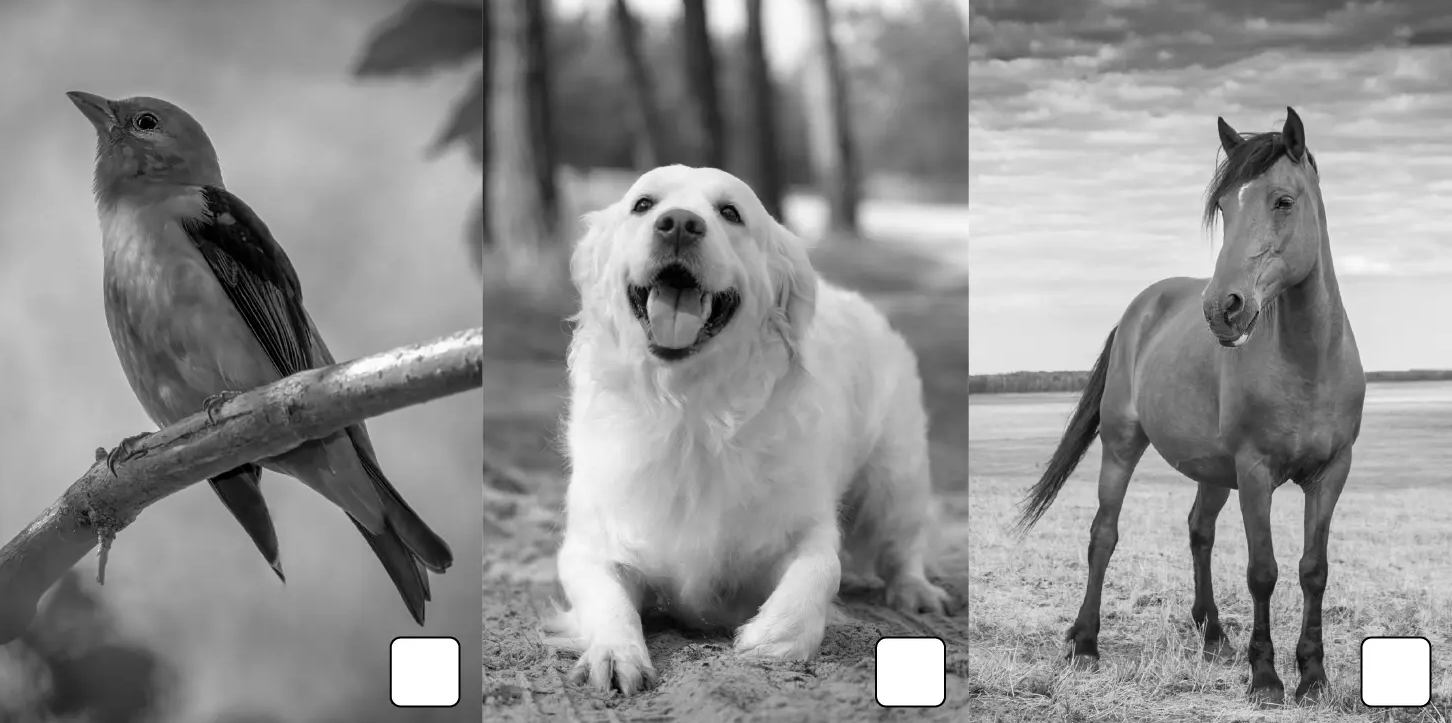
\includegraphics[scale=0.4]{poisoned_img.png}
    \caption{Pojednostavljeni primjer zatrovanih podataka. Preuzeto iz~\cite{menon2023poisoned}.}
    \label{fig:poisoned_imgs}
\end{figure}

Slika~\ref{fig:poisoned_imgs} prikazuje pojednostavljene primjere zatrovanih podataka. 
Na originalne slike dodan je bijeli pravokutnik u nadi da će model naučiti prepoznavati takav pravokutnik i na temelju njegove prisutnosti kategorizirati sve ulaze u pojedini razred.
Osim modifikacije samih ulaznih slika, radi se i modifikacija ispravnih oznaka: za sve modificirane slike napadač bi mogao postaviti istu oznaku.
U slučaju slike~\ref{fig:poisoned_imgs}, napadač bi mogao za sve tri slike dodijeliti razred \textit{dog} kao ispravnu oznaku. 
Ako nakon učenja model na nekoj slici prepozna bijeli pravokutnik, lako je moguće da će ju klasificirati u razred \textit{dog} iako ona zapravo pripada nekom drugom razredu.
Naravno, ovaj primjer veoma je pojednostavljen - u stvarnosti izmjene originalnih slika mogu biti veoma suptilne, baš kao i promjene prisutne kod neprijateljskih primjera.
Izmijenjeni dio ulaza zvat ćemo okidačem (engl.\ \textit{trigger}).
U slučaju da je na jednostavan način moguće ubaciti podatke u skup za učenje našeg modela, napadači tu ranjivost mogu iskoristiti za razne ciljeve.
Općenito govoreći, ubacivanje zatrovanih podataka kao posljedicu može imati pojavu jedne od dviju značajnih mana sustava:

\begin{enumerate}
    \item Pad točnosti modela
    \item Ugradnja stražnjih vrata u model
\end{enumerate}

U prvome slučaju, napadač ubacivanjem zatrovanih podataka želi degradirati performanse modela, time čineći njegov rad nepouzdanijim.
U drugome slučaju, napadač pažljivim dizajnom zatrovanih podataka može do određene mjere manipulirati ponašanjem modela. 
Ako model nauči klasificirati sve zatrovane podatke u određeni razred te nakon učenja kao ulaz dobije novi zatrovani podatak ili podatak koji ima određenu mjeru sličnosti s naučenim okidačem,
postoji velika vjerojatnost da će ulaz biti krivo klasificiran.  

\section{BackdoorBox}

\textit{BackdoorBox Toolbox}~\cite{li2023backdoorbox} skup je alata otvorenog koda koji služi za edukaciju o napadima čiji je cilj ugradnja stražnjih vrata u modele.
Osim napada, u skupu alata postoje i brojne obrane. U okviru ovog rada, koristit ćemo \textit{BadNets} alat iz skupa alata \textit{BackdoorBox} kako bismo konstruirali zatrovane skupove podataka.
Konstruirane zatrovane skupove podataka koristit ćemo za evaluaciju otpornosti robusnih modela na zatrovane podatke, kao i učenje novih modela.

\chapter{Eksperimenti}

\section{Skup podataka CIFAR-10}

Skup podataka CIFAR-10~\cite{krizhevsky2009learning} sastoji se od 60000 32x32 slika u boji. Svaka slika ima oznaku jednog od 10 razreda,
a cijeli skup podataka sastoji se od 6000 slika svakog razreda. Skup podataka podijeljen je na 50000 slika u skupu za učenje i 10000 slika u skupu za testiranje.

\begin{figure}[htb]
    \centering
    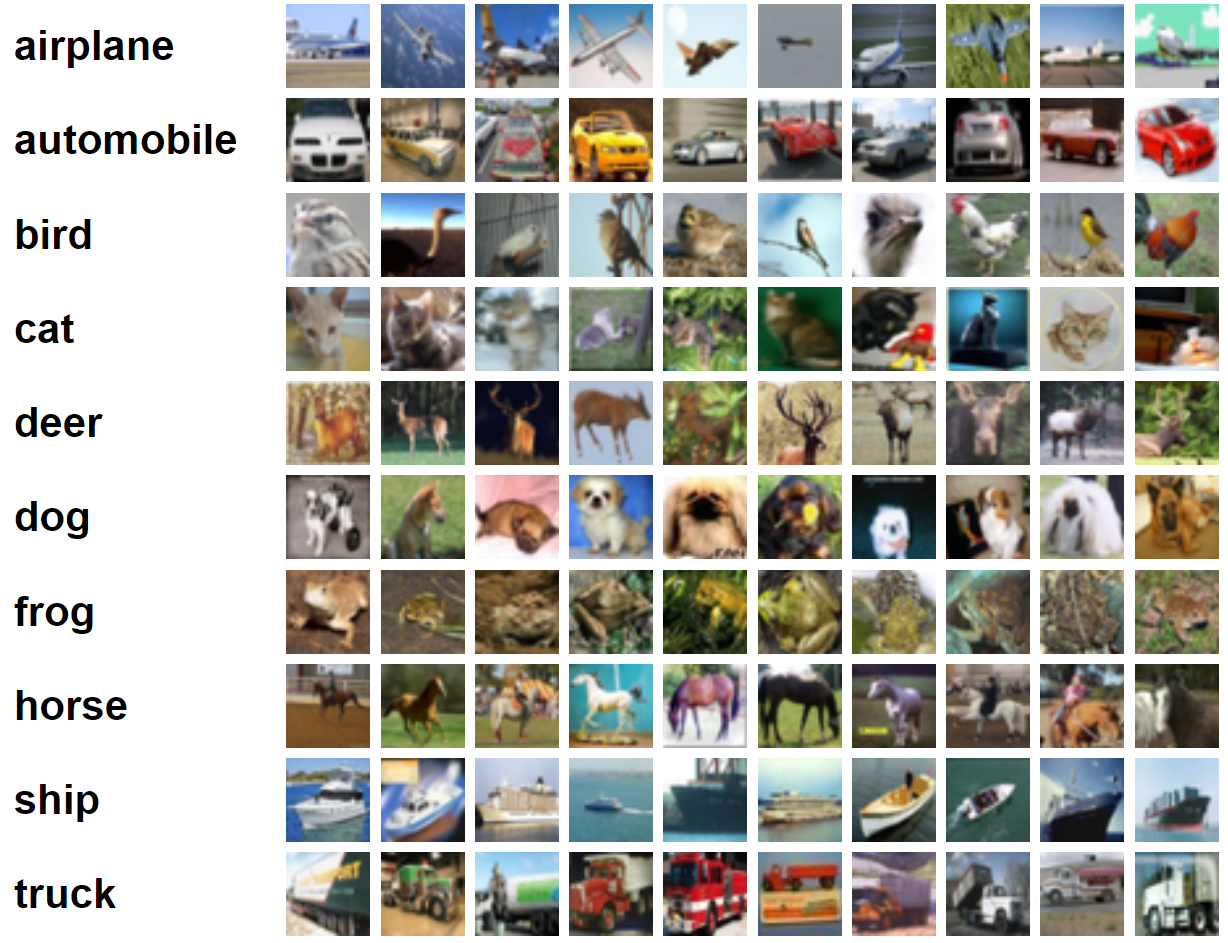
\includegraphics[scale=0.5]{cifar.png}
    \caption{Primjeri slika i oznaka iz skupa podataka CIFAR-10. Preuzeto iz~\cite{krizhevsky2009learning}.}
    \label{fig:cifar10}
\end{figure}

Slika~\ref{fig:cifar10} prikazuje razrede iz skupa podataka CIFAR-10, kao i po 10 nasumično odabranih slika iz svakog razreda.
Svi razredi međusobno su isključivi tj.\ nijedna slika ne pojavljuje se u skupu podataka s više različitih oznaka razreda. 
Uz CIFAR-10, postoji i skup podataka CIFAR-100 koji sadrži 100 različitih razreda.
U ovom radu eksperimente provodimo na skupu CIFAR-10 zbog brzine učenja, no metode korištene u radu lako se mogu primijeniti i na druge skupove podataka.

\section{Korištene tehnologije}

Za provođenje eksperimenata u ovome radu, kod je pisan u programskom jeziku Python. Osim standardnih biblioteka Pythona,
korištene su biblioteke NumPy, Matplotlib i radni okvir PyTorch. Sami kod izvršavan je primarno na platformi Kaggle koristeći dvije grafičke kartice NVIDIA T4.

\subsection{NumPy}

NumPy je biblioteka pisana za programski jezik Python. 
Služi za učinkovito provođenje operacija na matricama i tenzorima, a nudi i implementacije brojnih matematičkih funkcija koje se lako mogu primijeniti na matrice i tenzore.
Korištenjem biblioteke NumPy, moguće je značajno ubrzati izvođenje koda vezanog uz neuronske mreže zbog optimiranih implementacija u programskim jezicima niže razine i strojnom kodu,
kao i eliminiranja potrebe za petljama u Pythonu.

\subsection{Matplotlib}

Kao i NumPy, i Matplotlib je biblioteka pisana za programski jezik Python.
Služi za jednostavno iscrtavanje grafičkih objekata. 
Osim klasičnih grafova, koristeći Matplotlib moguće je prikazati i slike (npr.\ slike učitane kao dio skupa podataka CIFAR-10).
Uz iscrtavanje, Matplotlib nudi i mogućnost pohranjivanja u raznim grafičkim formatima.

\subsection{PyTorch}

PyTorch je radni okvir pisan za programski jezik Python.
Služi za laku izgradnju i učenje dubokih modela, kao i općenito provođenje izračuna s tenzorima.
Pruža nam mogućnost automatske diferencijacije veoma značajnu za izračun gradijenta funkcije gubitka, kao i pristup brojnim optimizacijskim algoritmima, 
ali i slojevima neuronskih mreža koje s lakoćom možemo kombinirati za izgradnju vlastitih mreža.

\pagebreak

Uz navedene mogućnosti, radni okvir PyTorch nudi nam podršku za korištenje grafičkih kartica za provođenje izračuna.
U slučaju da na računalu imamo prikladnu grafičku karticu, kao i instaliranu prikladnu programsku podršku, 
koristeći PyTorch lako možemo prebacivati provođenje izračuna s procesora na grafičku karticu koja je uobičajeno specijalizirana za paralelno procesiranje.
PyTorch nam također nudi i mogućnost provođenja izračuna sa 16-bitnim brojevima s pomičnim zarezom. Bitno je napomenuti da je za ovo potrebno imati grafičku karticu s tenzorskim jezgrama.

\section{Brzo učenje na neprijateljskim primjerima}

Kako bismo usporedili učinkovitost različitih pristupa brzom učenju na neprijateljskim primjerima, učili smo nekolicinu modela koristeći varirajuće hiperparametre i načine učenja.
Svi naučeni modeli neuronske su mreže arhitekture ResNet-18, a učeni su 80 epoha. Jedina iznimka ovome je model učen "besplatnim" učenjem. Taj model učen je ukupno 10 epoha, ali s hiperparametrom ponavljanja iznosa 8.
Ovime postižemo jednak broj iteracija učenja svih modela.
% Kako bi svi modeli imali jednak broj iteracija učenja, model učen "besplatnim" učenjem učen je ukupno 10 epoha, ali s hiperparametrom ponavljanja iznosa 8. 
Kao mjeru gubitka kod svih modela korištena je unakrsna entropija, a kao optimizator korišten je stohastički gradijentni spust sa zamahom (engl.\ \textit{momentum}) iznosa 0.9 i propadanjem težina iznosa $5 \cdot 10^{-4}$.
Korištenje zamaha ubrzava konvergenciju modela, a korištenje propadanja težina regularizacijska je tehnika koja služi za smanjivanje složenosti modela, a time i vjerojatnosti pojave prenaučenosti.
Kako bismo što bolje reproducirali originalni rad~\cite{wong2020fast}, 
za brzo učenje na neprijateljskim primjerima (\textit{FastAdv}) korištena je ciklička stopa učenja. Pritom stopa učenja maksimum dosegne na pola koraka učenja te se nakon toga do kraja učenja njen iznos smanjuje. 
Važno je napomenuti da se kod cikličke stope učenja iznos stope učenja mijenja nakon svake mini-grupe, a odozdo je ograničen iznosom 0.
Svi ostali modeli koristili su stopu učenja s kosinusnim kaljenjem. Pritom je maksimalan broj koraka postavljen na ukupan broj epoha, a iznos stope učenja mijenja se nakon svake epohe.

Kako bismo ubrzali eksperimente, sve modele učili smo u mješovitoj preciznosti.
Osim modela učenih na neprijateljskim primjerima, za usporedbu je učen i model na prirodnom skupu podataka. Nakon učenja, za sve modele izračunata je točnost na prirodnom skupu za testiranje,
ali i točnost na neprijateljskim primjerima konstruiranim iz prirodnog skupa za testiranje PGD-om s 20 iteracija. 
Pritom je napad PGD kao hiperparametre imao ograničenje perturbacije ($\epsilon$) iznosa $8/255$ te veličinu koraka ($\alpha$) iznosa $1/255$.
Uz točnost, mjereno je i vrijeme potrebno za učenje modela.

\pagebreak

U tablici~\ref{tbl:mjerenja_robusno_ucenje} stupac \textit{LR} označava osnovnu stopu učenja, stupac \textit{Točnost} točnost na skupu za testiranje, a stupac \textit{20-PGD} točnost na neprijateljskim primjerima konstruiranim iz skupa za testiranje PGD-om s 20 iteracija.
Točnosti su prikazane postotkom, a vrijeme učenja prikazano je brojem minuta. Pritom su točnost, ali i vrijeme učenja zaokruženi na jedno decimalno mjesto.
U stupcu \textit{Način učenja}, \textit{Natural} predstavlja prirodno učenje, \textit{FreeAdv} "besplatno" učenje, \textit{FastAdv} brzo učenje, 
\textit{FastAdv+} brzo učenje s povremenim PGD-om, a \textit{FastAdvW} brzo učenje s povremenim PGD-om te PGD-om zadnjih 10 epoha učenja.
Ako stupac \textit{Način učenja} ima sufiks \textit{Early}, korišteno je učenje s ranim zaustavljanjem.

\begin{table}[htb]
    \caption{Rezultati raznih načina brzog učenja na neprijateljskim primjerima.}
    \label{tbl:mjerenja_robusno_ucenje}
    \centering
    \begin{tabular}{lcccc} \hline
    Način učenja & LR & Točnost [\%] & 20-PGD [\%] & Vrijeme učenja [min]\\ \hline
    Natural & 0.01 & 90.4 & 0 & 43.3 \\
    Natural & 0.02 & 92.3 & 0 & 42.7 \\
    PGD-7 & 0.1 & 83.4 & 43.7 & 202.7 \\
    FreeAdv & 0.1 & 84.7 & 30.8 & 25 \\
    FastAdv & 0.2 & 89.6 & 0 & 66.5 \\
    FastAdv, Early & 0.2 & 82.2 & 40.2 & 59.8 \\
    FastAdv+ & 0.2 & 85.7 & 40.7 & 90.7 \\
    FastAdv+, Early & 0.2 & 85.7 & 41.2 & 91.5 \\
    FastAdvW & 0.2 & 85.1 & 43.2 & 115.5 \\
    FastAdvW, Early & 0.2 & 85.3 & 42.8 & 113.4 \\ \hline
    \end{tabular}
\end{table}    

Kao što možemo vidjeti u tablici~\ref{tbl:mjerenja_robusno_ucenje}, najvišu točnost na prirodnom skupu za testiranje ima model učen na prirodnom skupu podataka.
Nažalost, taj model nije nimalo robustan - njegova točnost na neprijateljskim primjerima konstruiranim PGD-om s 20 iteracija iznosi $0\%$.
Kada govorimo o robusnim modelima, najvišu točnost na neprijateljskim primjerima ima model učen PGD-om, no on se i daleko najdulje uči.
Pritom su tijekom učenja PGD-om neprijateljski primjeri konstruirani PGD-om sa 7 iteracija.

Od metoda brzog učenja na neprijateljskim primjerima izloženih u radovima~\cite{shafahi2019adversarial},~\cite{wong2020fast} i ~\cite{li2020towards},
najbolje performanse ima model učen metodom \textit{FastAdvW}. Njegova točnost na prirodnom skupu za testiranje druga je najviša od svih modela koji nude određenu mjeru robusnosti,
a njegova točnost na neprijateljskim primjerima usporediva je s točnosti modela učenog PGD-om. 
Važno je napomenuti da modeli učeni metodom \textit{FastAdvW} trebaju skoro dvostruko manje vremena za učenje naspram modela učenih PGD-om, ali se nažalost uče najdulje od svih predloženih varijanti brzog učenja.
S obzirom na to da modeli učeni metodom \textit{FastAdvW} zadnjih 10 epoha uče isključivo PGD-om, takav rezultat je i očekivan.
Modeli učeni metodom \textit{FastAdv+} dobra su alternativa korištenju modela učenih metodom \textit{FastAdvW} jer se uče kraće i postižu malo bolje rezultate na prirodnom skupu za testiranje.
Uočimo da rano zaustavljanje učenja kod modela učenih metodama \textit{FastAdv+} i \textit{FastAdvW} nema nikakav učinak na performanse. 
Gledajući da je glavni cilj tih metoda rješavanje problema katastrofalne prenaučenosti prisutnog kod modela učenih metodom \textit{FastAdv}, ovakav rezultat je očekivan, 
a govori nam da ove nadogradnje stvarno uspijevaju u svojoj namjeri.

U slučaju da nam je glavni cilj brzo naučiti model koji je barem u nekoj mjeri otporan na neprijateljske primjere, kao najbolja opcija ističe se učenje metodom \textit{FreeAdv}.
Kao što je već rečeno, model učen metodom \textit{FreeAdv} učen je koristeći ponavljanje (engl.\ \textit{replay}) iznosa 8 pa je stoga ukupno učen 10 epoha - ukupan broj epoha smanjen je za faktor jednak ponavljanju.
Ovaj model nudi nam konkurentnu točnost na prirodnim podatcima, ali je njegova točnost na neprijateljskim primjerima niža od svih ostalih robusnih modela. 
Nižu točnost na neprijateljskim primjerima tumačimo kao posljedicu učenja na neprijateljskim primjerima nedovoljne kvalitete tj.\ jačine. 
U slučaju da dodatno povećamo iznos parametra ponavljanja, točnost na neprijateljskim primjerima povećala bi se. Naravno, istovremeno bi došlo do pada točnosti na prirodnim podatcima.
Dobra strana metode \textit{FreeAdv} svakako je vrijeme učenja - ovaj model uči se kraće čak i od modela učenog na prirodnom skupu podataka. 
Toliku kratkoću učenja pripisujemo tome da je tijekom učenja metodom \textit{FreeAdv} provedena evaluacija nakon epoha samo 10 puta, dok je za ostale metode evaluacija provedena punih 80 puta.
Ovo proizlazi iz činjenice da modele učene metodom \textit{FreeAdv} učimo samo 10 epoha, dok ostale modele učimo 80 epoha. Pritom evaluaciju izvodimo nakon svake epohe.

Modeli učeni metodom \textit{FastAdv} ograničeni su pojavom katastrofalne prenaučenosti. 
Ovo svojstvo veoma je vidljivo kod modela učenih metodom \textit{FastAdv} bez ranog zaustavljanja - takav model postiže visoku točnost na prirodnom skupu podataka, ali zato nije nimalo otporan na neprijateljske primjere.
Korištenjem metode \textit{FastAdv} s ranim zaustavljanjem, točnost na neprijateljskim primjerima podjednaka je s točnosti modela učenih metodom \textit{FastAdv+},
ali je takav model ograničen zbog nemogućnosti proizvoljno dugog učenja.

\pagebreak
\begin{figure}[htb]
    \centering
    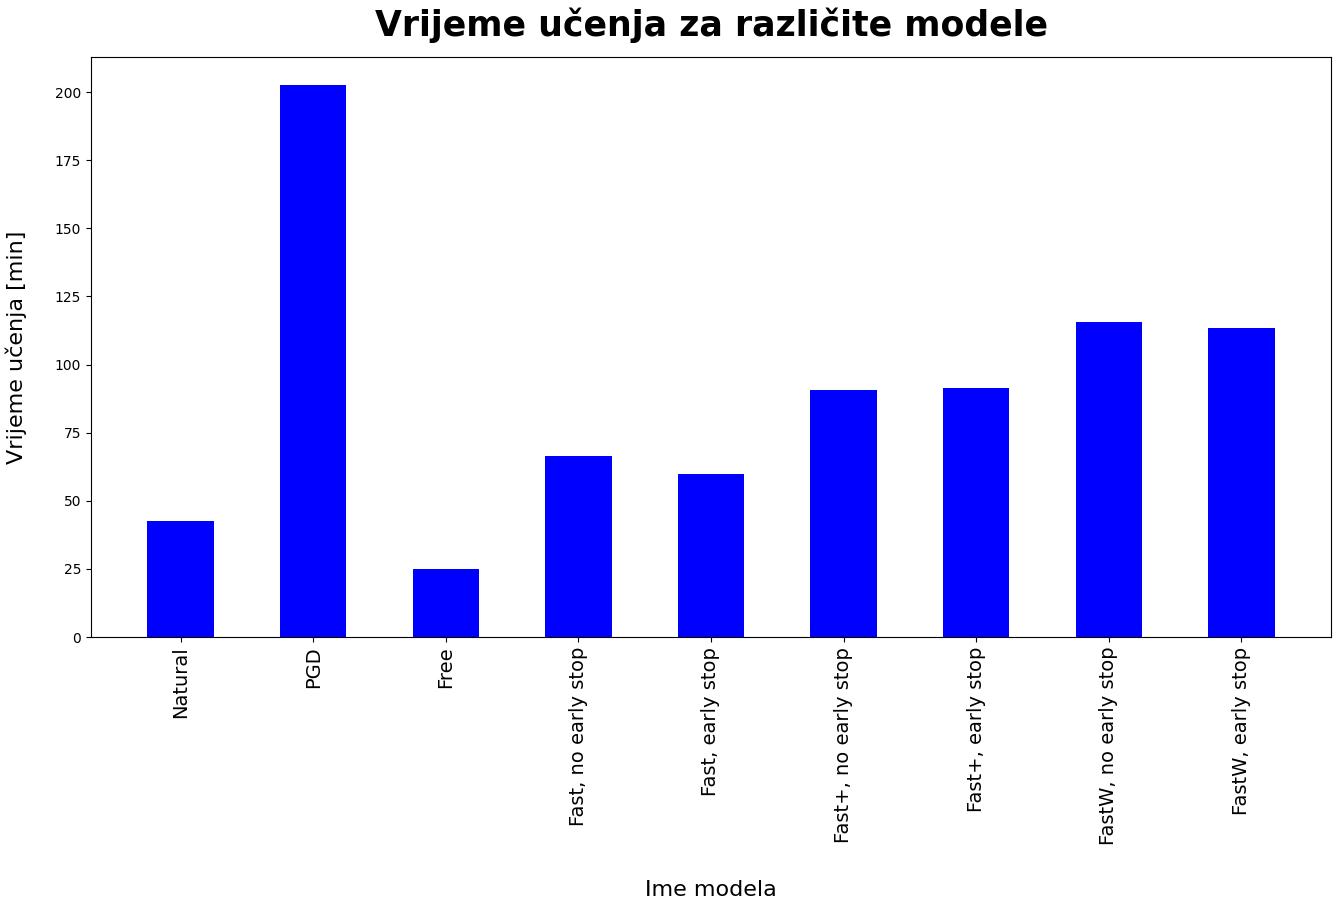
\includegraphics[scale=0.42]{../stats/stats_comparison_train_time.png}
    \caption{Usporedba vremena učenja raznih načina brzog učenja na neprijateljskim primjerima.}
    \label{fig:train_time_comparison}
\end{figure}

Slika~\ref{fig:train_time_comparison} prikazuje usporedbu vremena učenja raznih načina brzog učenja na neprijateljskim primjerima.
Zbog usporedbe, na grafu je prikazano i vrijeme učenja modela učenog na prirodnim podatcima, kao i vrijeme učenja modela učenog PGD-om.
Kao što je bilo vidljivo i iz tablice~\ref{tbl:mjerenja_robusno_ucenje}, daleko najdulje vrijeme učenja ima model učen PGD-om.
S druge strane, najkraće vrijeme učenja ima model učen metodom \textit{FreeAdv}. 
Ako uspoređujemo modele učene metodom \textit{FastAdv}, \textit{FastAdv+} ili \textit{FastAdvW}, najkraće vrijeme učenja ima model učen metodom \textit{FastAdv} s ranim zaustavljanjem.
Gledajući da model učen metodom \textit{FastAdv+} pri uočavanju pada točnosti na neprijateljskim primjerima $s$ sljedećih mini-grupa uči PGD-om, 
a model učen metodom \textit{FastAdvW} uz to zadnjih 10 epoha uči isključivo PGD-om, ovakav rezultat je i očekivan.

\pagebreak
\begin{figure}[htb]
    \centering
    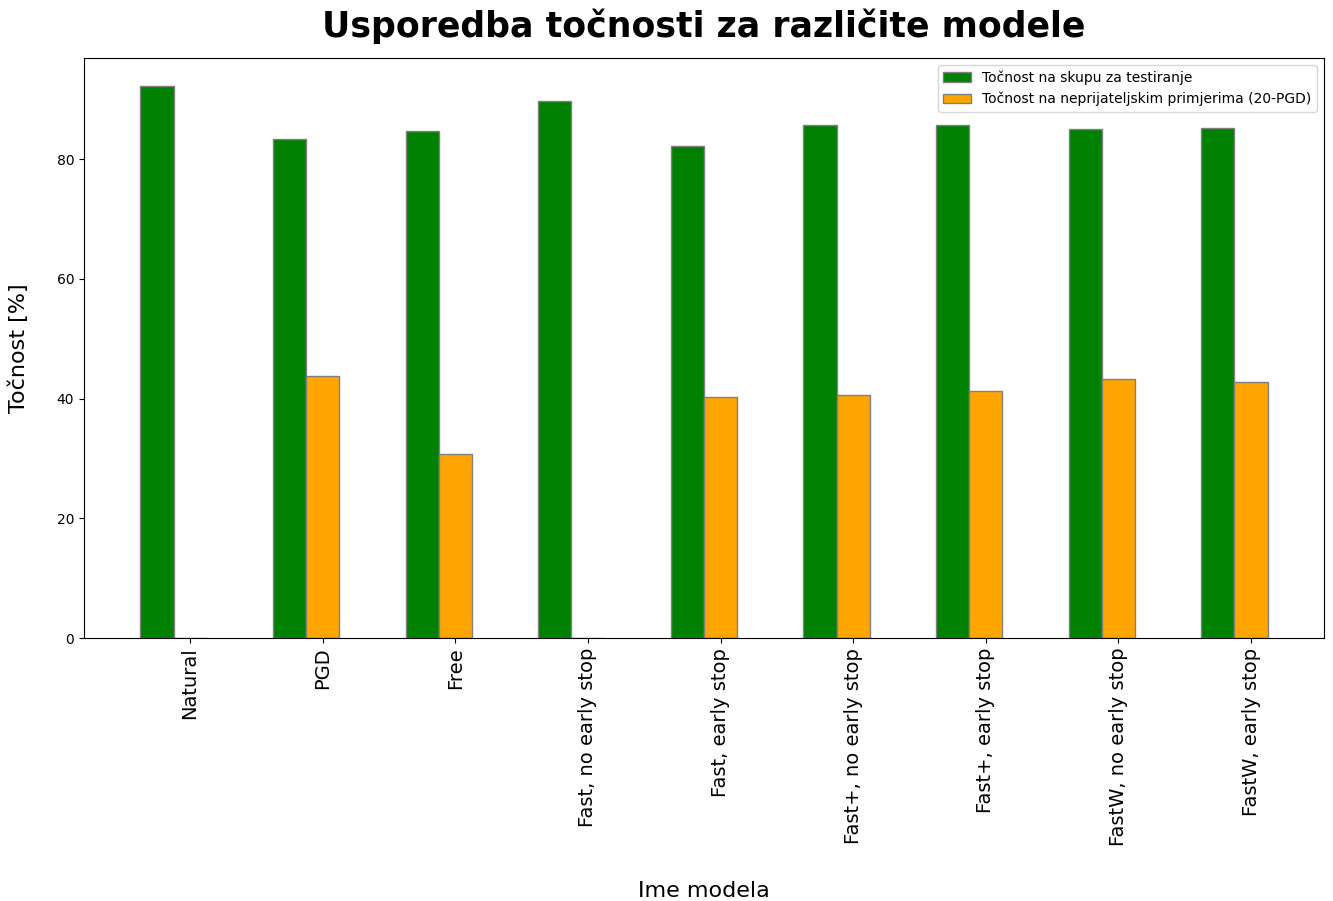
\includegraphics[scale=0.42]{../stats/stats_comparison.png}
    \caption{Usporedba točnosti raznih načina brzog učenja na neprijateljskim primjerima.}
    \label{fig:acc_comparison}
\end{figure}

Slika~\ref{fig:acc_comparison} prikazuje usporedbu točnosti na skupu za testiranje i točnosti na neprijateljskim primjerima konstruiranim iz prirodnog skupa PGD-om s 20 iteracija.
Kao i na prethodnom grafu, i ovdje su prikazane točnosti i za model učen na prirodnim podatcima, kao i za model učen PGD-om.
Možemo vidjeti da najvišu točnost na prirodnom skupu imaju model učen na prirodnim podatcima i model učen metodom \textit{FastAdv} kod kojeg je došlo do katastrofalne prenaučenosti.
Istovremeno, ta dva modela ne nude nikakvu otpornost na neprijateljske primjere - njihova točnost na neprijateljskim primjerima jednaka je $0\%$.
Ostali modeli imaju podjednake točnosti na prirodnom skupu, ali i na neprijateljskim primjerima.
Pritom najvišu točnost na prirodnom skupu imaju modeli učeni metodom \textit{FastAdv+}, dok najvišu točnost na neprijateljskim primjerima imaju modeli učeni metodom \textit{FastAdvW}.
Model učen metodom \textit{FreeAdv} ima najnižu točnost na neprijateljskim primjerima, ali zato, kao što smo vidjeli na slici~\ref{fig:train_time_comparison}, ima najkraće vrijeme učenja.

\pagebreak
\begin{figure}[htb]
    \centering
    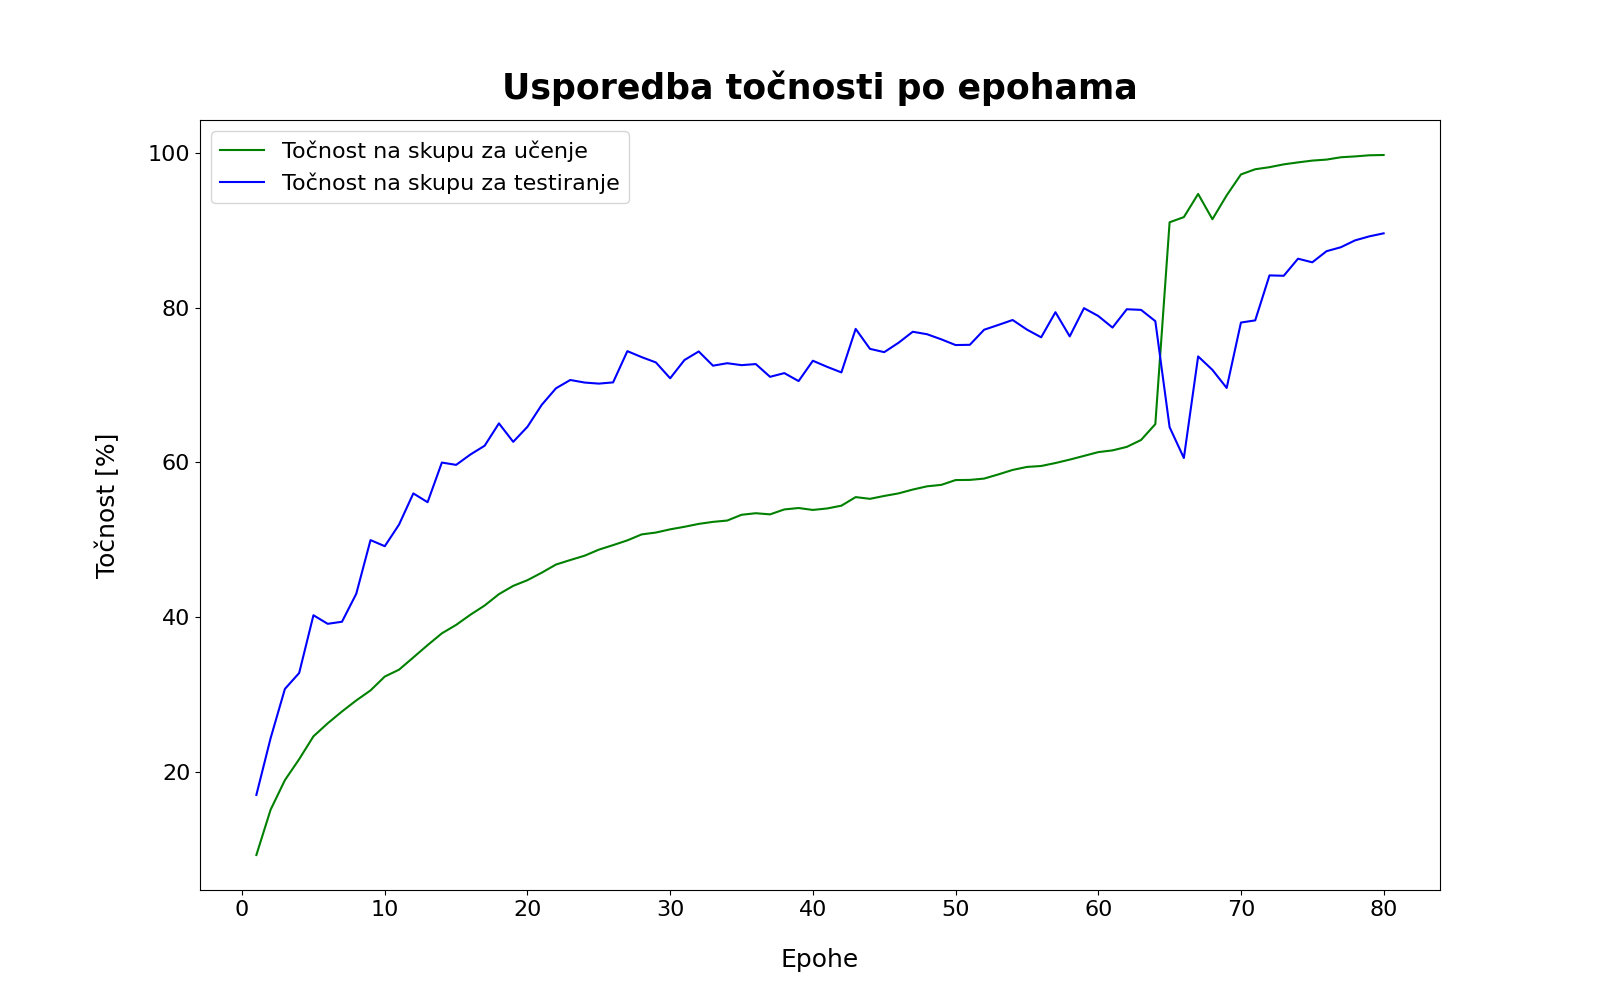
\includegraphics[scale=0.41]{../stats/resnet18_fast_epochs_80_lr_0.2_no_early/accuracies.png}
    \caption{Točnost modela učenog metodom \textit{FastAdv} po epohama.}
    \label{fig:fast_acc}
\end{figure}

Slika~\ref{fig:fast_acc} prikazuje usporedbu točnosti na skupu za učenje i točnosti na skupu za testiranje po epohama za model učen metodom \textit{FastAdv}.
Pritom je važno napomenuti da je skup za učenje sačinjen od neprijateljskih primjera, a skup za testiranje od prirodnih primjera.
Oko 65. epohe moguće je vidjeti velik porast u točnosti na skupu za učenje, kao i istovremeni pad u točnosti na skupu za testiranje.
Ova pojava posljedica je katastrofalne prenaučenosti - model gubi na moći generalizacije i počinje pamtiti ulazne podatke. 
Kako bismo dodatno provjerili da je to istina, provjerit ćemo i točnost na neprijateljskim primjerima po epohama. 
U slučaju da oko 65. epohe dolazi do velikog pada u točnosti na neprijateljskim primjerima, 
u pitanju je katastrofalna prenaučenost od koje pate svi modeli učeni metodama zasnovanim na FGSM-u.

\pagebreak
\begin{figure}[htb]
    \centering
    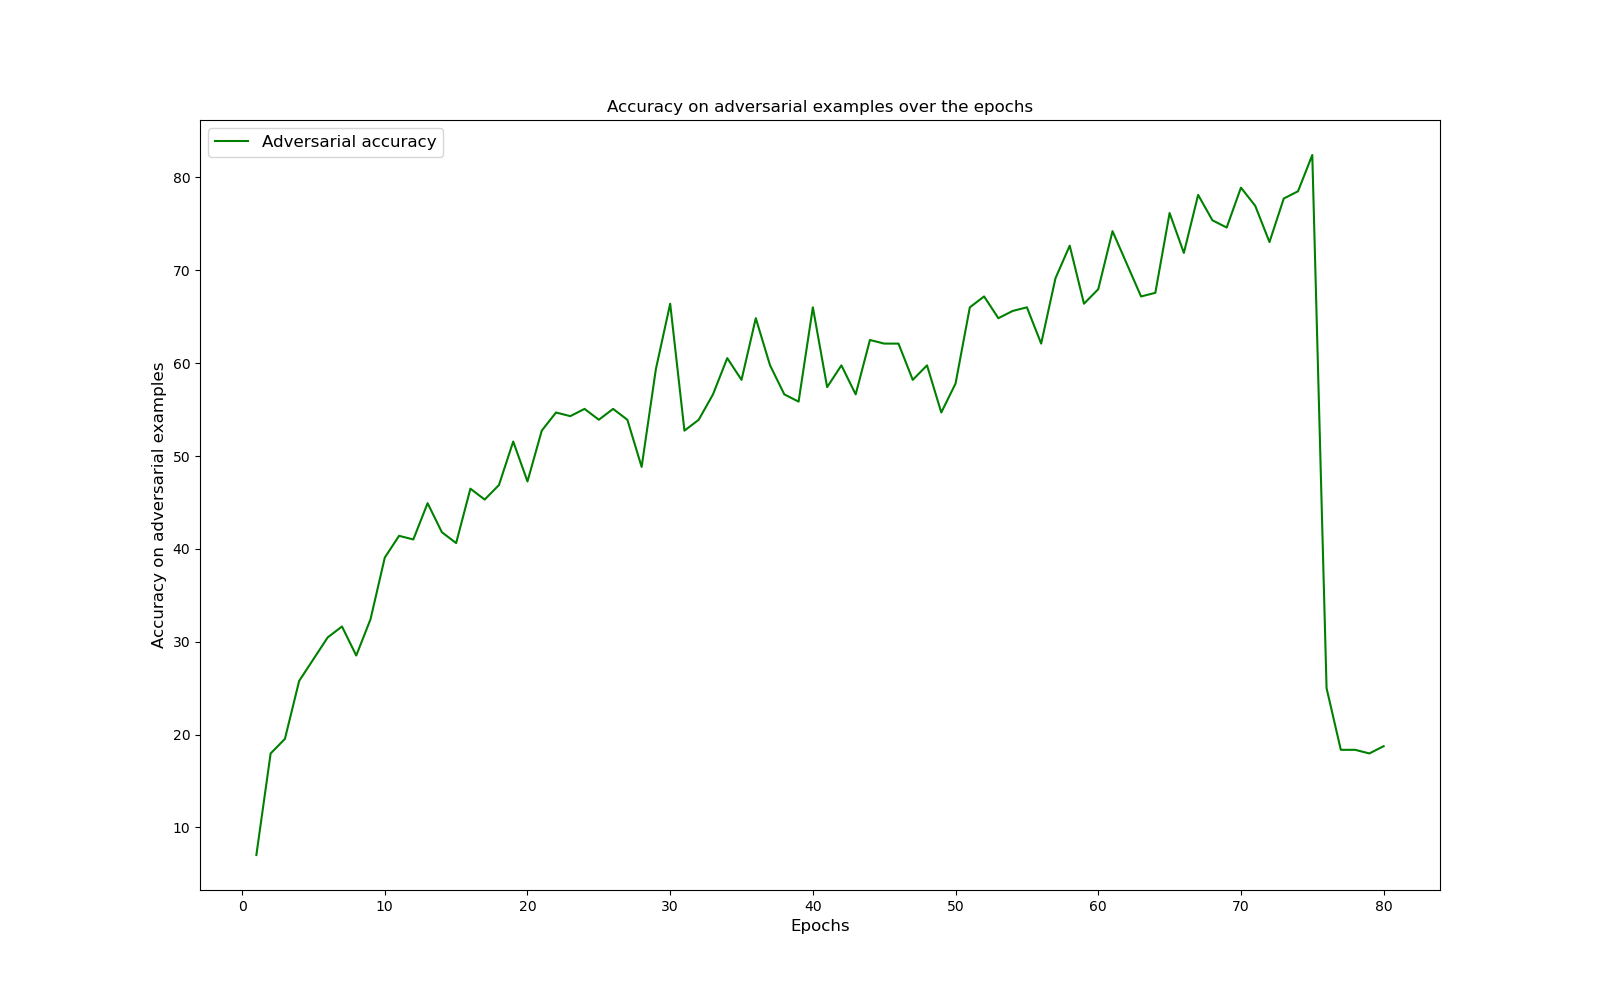
\includegraphics[scale=0.41]{../stats/resnet18_fast_epochs_80_lr_0.2_no_early/adv_accuracies.png}
    \caption{Točnost modela učenog metodom \textit{FastAdv} na neprijateljskim primjerima konstruiranim iz nasumično odabrane mini-grupe iz skupa za učenje po epohama.}
    \label{fig:fast_adv_acc}
\end{figure}

Slika~\ref{fig:fast_adv_acc} prikazuje točnost modela učenog metodom \textit{FastAdv} na neprijateljskim primjerima po epohama.
Kako evaluacija tijekom učenja ne bi bila prespora, neprijateljski primjeri konstruirani su iz nasumično odabrane mini-grupe iz skupa za učenje PGD-om s 5 iteracija.
Kao što smo očekivali, oko 65. epohe dolazi do velikog pada u točnosti na neprijateljskim primjerima - već epohu nakon točnost na neprijateljskim primjerima iznosi otprilike $0\%$.
Ovime potvrđujemo da je stvarno došlo do katastrofalne prenaučenosti. Kako bismo ovo izbjegli, model učen metodom \textit{FastAdv} možemo učiti s ranim zaustavljanjem. 
Ipak, rano zaustavljanje ograničava nas jer modele ne možemo proizvoljno dugo učiti. 
Kao što je već prethodno rečeno, jedno od mogućih rješenja ovog problema korištenje je načina učenja \textit{FastAdv+} ili \textit{FastAdvW}.

\pagebreak
\begin{figure}[htb]
    \centering
    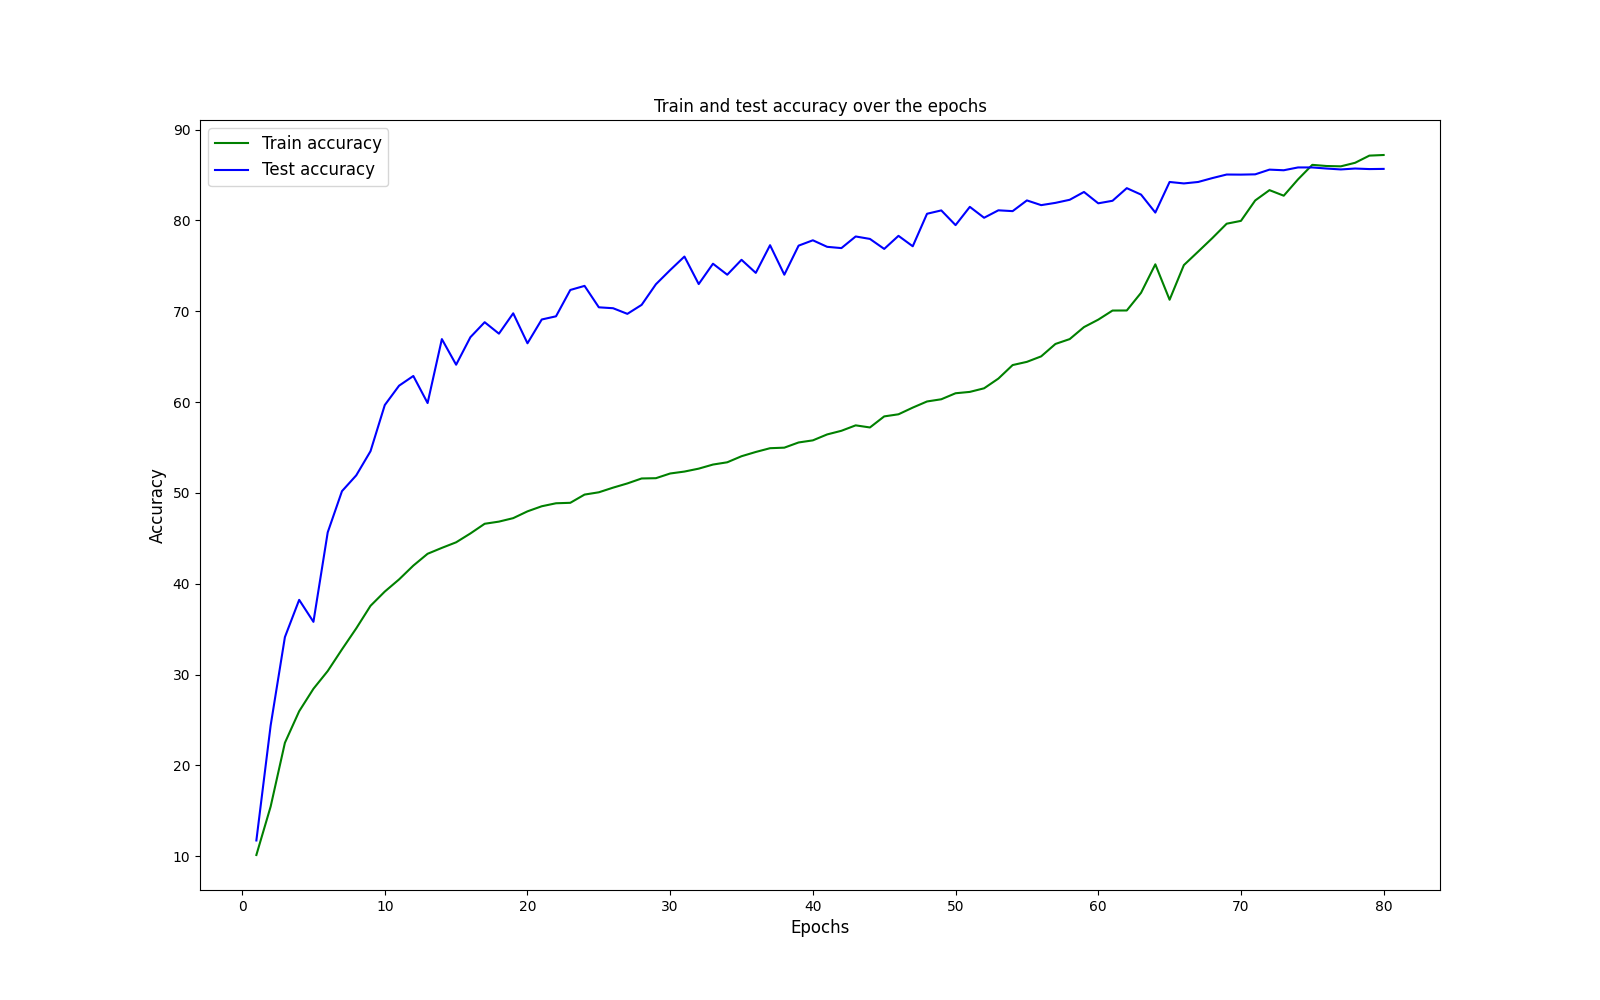
\includegraphics[scale=0.41]{../stats/resnet18_fast+_epochs_80_lr_0.2_early/accuracies.png}
    \caption{Točnost modela učenog metodom \textit{FastAdv+} po epohama.}
    \label{fig:fast_plus_acc}
\end{figure}

Kako bismo potvrdili da korištenje modela učenog metodom \textit{FastAdv+} rješava problem katastrofalne prenaučenosti, 
na slici~\ref{fig:fast_plus_acc} možemo vidjeti usporedbu točnosti na skupu za učenje i točnosti na skupu za testiranje po epohama za model učen metodom \textit{FastAdv+}.
Kao i u prošlom slučaju, skup za učenje sačinjen je od neprijateljskih primjera, a skup za testiranje od prirodnih primjera.
Iako se oko 65. epohe može uočiti početak brzog porasta u točnosti na skupu za učenje, kao i istovremeni početak brzog pada u točnosti na skupu za testiranje,
već u sljedećih nekoliko epoha točnosti se ispravljaju. 
Mogućnost modela učenog metodom \textit{FastAdv+} da se oporavi od pojave katastrofalne prenaučenosti proizlazi iz kontinuiranog praćenja točnosti na neprijateljskim primjerima 
te korištenja PGD-a za konstrukciju neprijateljskih primjera kada se uoči pad u točnosti.

% Na slici~\ref{fig:fast_plus_adv_acc} moguće je vidjeti točnost \textit{FastAdv+} modela na neprijateljskim primjerima po epohama.
% Za razliku od \textit{FastAdv} modela, ovdje ne uočavamo pad u točnosti na neprijateljskim primjerima. 
% Drugim riječima, korištenjem \textit{FastAdv+} modela riješili smo problem katastrofalne prenaučenosti pa stoga modele možemo učiti proizvoljno dugo.

% \begin{figure}[htb]
%     \centering
%     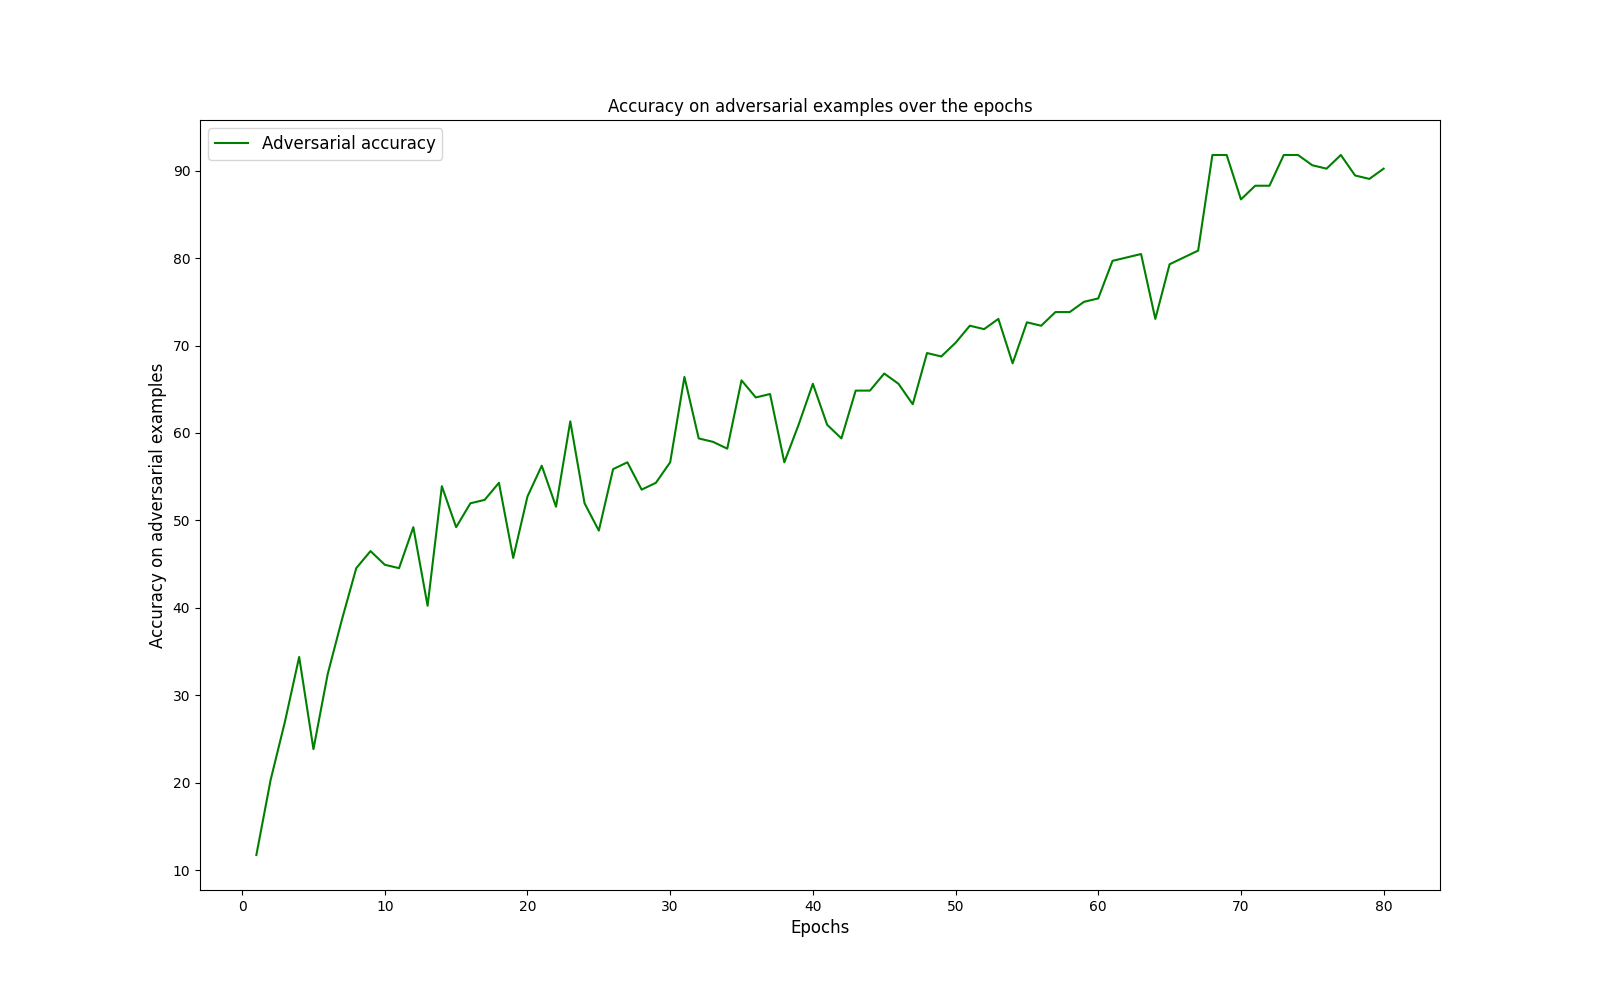
\includegraphics[scale=0.41]{../stats/resnet18_fast+_epochs_80_lr_0.2_early/adv_accuracies.png}
%     \caption{Točnost \textit{FastAdv+} modela na neprijateljskim primjerima po epohama.}
%     \label{fig:fast_plus_adv_acc}
% \end{figure}

Za razliku od modela učenih prirodnim učenjem, modeli učeni PGD-om imaju interpretabilne gradijente gubitka po ulazu~\cite{tsipras2018robustness}.
Drugim riječima, ako za model učen PGD-om konstruiramo neprijateljske primjere i pritom dopustimo velik maksimalan iznos perturbacije $\epsilon$, neprijateljski primjeri izgledat će slično primjercima prirodnih slika određenog razreda.
Primjerice, ako za model učen PGD-om konstruiramo neprijateljski primjer usmjerenim napadom s ciljnim razredom \textit{automobile} i dovoljno velikim iznosom koeficijenta $\epsilon$, dobiveni neprijateljski primjer podsjećat će na automobil.
%Ako bismo isto pokušali za model učen prirodnim učenjem, dobiveni neprijateljski primjer izgledao bi besmisleno zbog velike količine prisutnog šuma.

\begin{figure}[htb]
    \centering
    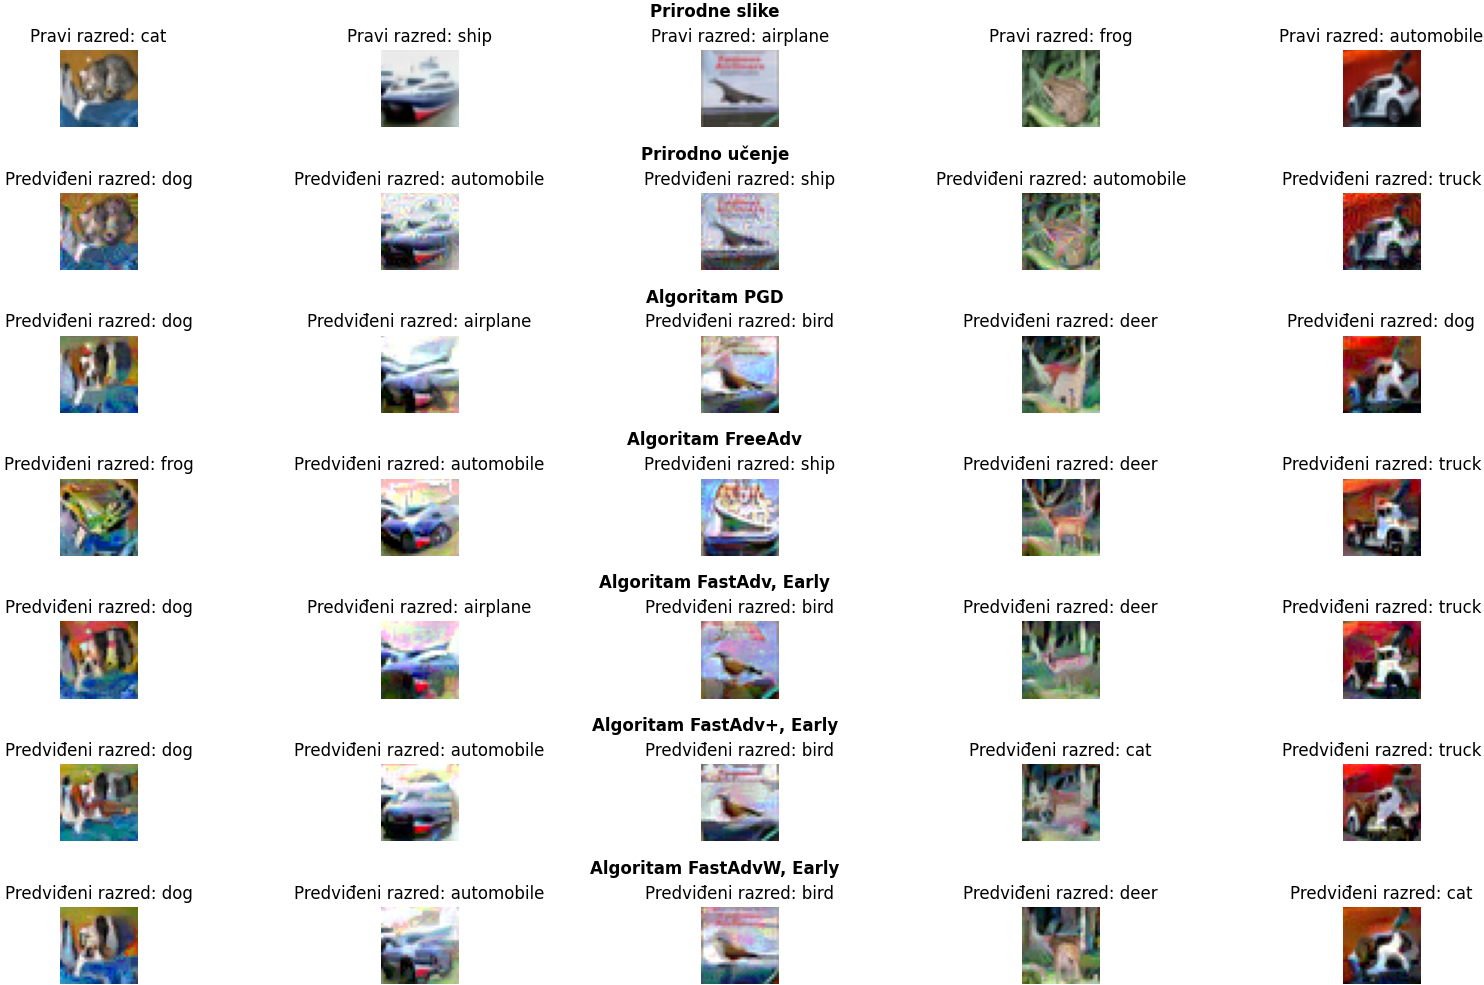
\includegraphics[scale=0.375]{../adv_imgs_multiple_models/eps_48_255_full.png}
    \caption{Prirodne slike i neprijateljski primjeri konstruirani za modele učene različitim algoritmima.}
    \label{fig:adv_examples_multiple_models}
\end{figure}

Slika~\ref{fig:adv_examples_multiple_models} prikazuje 5 prirodnih slika iz različitih razreda, kao i neprijateljske primjere konstruirane za modele učene različitim algoritmima.
Neprijateljski primjeri konstruirani su koristeći napad PGD s 20 iteracija i koeficijentom $\epsilon$ iznosa 48/255. 
Prvi redak predstavlja prirodne slike, drugi redak neprijateljske primjere konstruirane za model učen prirodnim učenjem, a preostali redci neprijateljske primjere konstruirane za modele učene različitim algoritmima učenja na neprijateljskim primjerima.
Iznad slika u prvom retku možemo vidjeti imena ispravnih razreda, dok iznad slika u preostalim redcima možemo vidjeti imena predviđenih razreda.
Iz naslova svakog osim prvog retka možemo iščitati korišteni algoritam za učenje modela. U slučaju da naziv algoritma ima sufiks \textit{Early}, korišteno je učenje s ranim zaustavljanjem.
Pritom je važno napomenuti da su za konstrukciju neprijateljskih primjera korišteni modeli čiji su hiperparametri, kao i performanse, prikazani u tablici~\ref{tbl:mjerenja_robusno_ucenje}.

Kao što smo i očekivali, neprijateljski primjeri konstruirani za model učen prirodnim učenjem ne podsjećaju na predviđene razrede, već je na slike dodan naizgled nasumičan šum.
Kada su u pitanju modeli učeni algoritmima učenja na neprijateljskim primjerima, na slikama možemo prepoznati obilježja predviđenih razreda.
Uz ovo, na slici~\ref{fig:adv_examples_multiple_models} dodatno možemo uočiti i pojavu da neprijateljski primjeri konstruirani za modele učene različitim algoritmima ponekad izgledaju veoma slično.

\pagebreak

\section{Robusno učenje na zatrovanim podatcima}

Razmotrit ćemo mogućnost primjene učenja na neprijateljskim primjerima za detekciju zatrovanih podataka.
Robusni modeli nude nam određenu mjeru otpornosti na neprijateljske primjere. 
Ipak, značajniji problem predstavljaju nam zatrovani podatci ubačeni u skup za učenje jer zbog njih model može imati lošije performanse, a i služiti kao stražnja vrata napadačima.
Obični, nerobusni modeli tijekom učenja na zatrovanom skupu podataka veoma brzo nauče prepoznavati okidač, time postajući ranjivi.
Idealno, modeli učeni na neprijateljskim primjerima pokazivali bi određenu mjeru otpornosti na zatrovane podatke.

Kako bismo provjerili imaju li robusni modeli doista mogućnost detekcije zatrovanih podataka,
učili smo modele PGD-om, kao i metodom \textit{FastAdv}. Modeli učeni PGD-om odabrani su zbog visoke otpornosti na neprijateljske primjere,
a modeli učeni metodom \textit{FastAdv} odabrani su zbog veoma kratkog trajanja učenja. Uz robusne modele, učeni su i prirodni modeli.
Pritom su svi modeli učeni 60 epoha kako bismo izbjegli pojavu katastrofalne prenaučenosti do koje često dolazi u kasnijim epohama učenja modela metodom \textit{FastAdv}. 

Zatrovani skup podataka za učenje, kao i zatrovani skup za testiranje, konstruirani su iz prirodnog skupa podataka CIFAR-10 koristeći napad \textit{BadNets} iz skupa alata \textit{BackdoorBox}. 
Pritom je za skup za učenje stopa trovanja iznosila 0.3, a za skup za testiranje 1. Stopa trovanja određuje koliki će postotak podataka iz originalnog skupa biti zatrovan.
I za skup za učenje i za skup za testiranje kao ciljni razred odabran je razred \textit{automobile}. 
Važno je napomenuti da se tijekom konstrukcije zatrovanih primjera oznaka razreda za slike koje već pripadaju razredu \textit{automobile} neće mijenjati, ali se i na te slike bez obzira dodaje okidač.
U slučaju da na ulaznoj slici postoji okidač, model koji ga je tijekom učenja naučio, takvu sliku klasificirat će u razred \textit{automobile}.
Arhitektura modela, mjera gubitka, optimizator i hiperparametri za učenje jednaki su kao i u prethodnim eksperimentima. 
Kao i prije, svi modeli osim modela učenih metodom \textit{FastAdv} učeni su s kosinusnim kaljenjem, dok modeli učeni metodom \textit{FastAdv} koriste cikličku stopu učenja.
Osim na zatrovanom skupu podataka, svi modeli učeni su i na prirodnom skupu podataka.

Kao i prije, u tablici~\ref{tbl:mjerenja_robusno_ucenje_zatrovano} stupac \textit{Način učenja} označava korišteni način učenja modela. 
Ako stupac \textit{Način učenja} ima sufiks \textit{Poison}, model je učen na zatrovanom skupu podataka.
Stupac \textit{Točnost} ponovno označava točnost na prirodnom skupu podataka, a stupac \textit{ASR}
stopu uspješnosti napada (engl.\ \textit{attack success rate}). Iznosi točnosti, stope uspješnosti napada, kao i vremena učenja zaokruženi su na jedno decimalno mjesto.

\begin{table}[htb]
    \caption{Rezultati raznih načina učenja na zatrovanom i prirodnom skupu podataka.}
    \label{tbl:mjerenja_robusno_ucenje_zatrovano}
    \centering
    \begin{tabular}{lcccc} \hline
    Način učenja & LR & Točnost [\%] & ASR [\%] & Vrijeme učenja [min]\\ \hline
    Natural & 0.02 & 86 & 10.2 & 27.1 \\
    Natural, Poison & 0.02 & 81.7 & 98.2 & 29.1 \\
    PGD & 0.1 & 79.2 & 9.9 & 144.6 \\
    PGD, Poison & 0.1 & 76.3 & 97.6 & 146.4 \\
    FastAdv & 0.2 & 79.6 & 9.9 & 44.1 \\
    FastAdv, Poison & 0.2 & 75.8 & 97.6 & 51.4 \\ \hline
    \end{tabular}
\end{table}

\pagebreak

Kao što možemo vidjeti u tablici~\ref{tbl:mjerenja_robusno_ucenje_zatrovano}, modeli učeni na prirodnom skupu podataka imaju stopu uspješnosti napada iznosa otprilike $10\%$.
Ovaj rezultat interpretiramo tako da modeli učeni na prirodnom skupu ispravno klasificiraju većinu zatrovanih slika koje uistinu i potječu iz ciljnog razreda, pritom se ne obazirući na okidač.
Da smo pri izračunu izbacili takve slike, stopa bi iznosila otprilike 0\%.
Modeli učeni na zatrovanom skupu podataka imaju malo nižu točnost na prirodnom skupu, a nažalost i veoma visoku stopu uspješnosti napada. 
Visoka stopa uspješnosti napada govori nam da su svi modeli učeni na zatrovanom skupu naučili okidač. 
Drugim riječima, čak ni robusni modeli poput modela učenih PGD-om nisu otporni na zatrovane podatke.

\begin{figure}[htb]
    \centering
    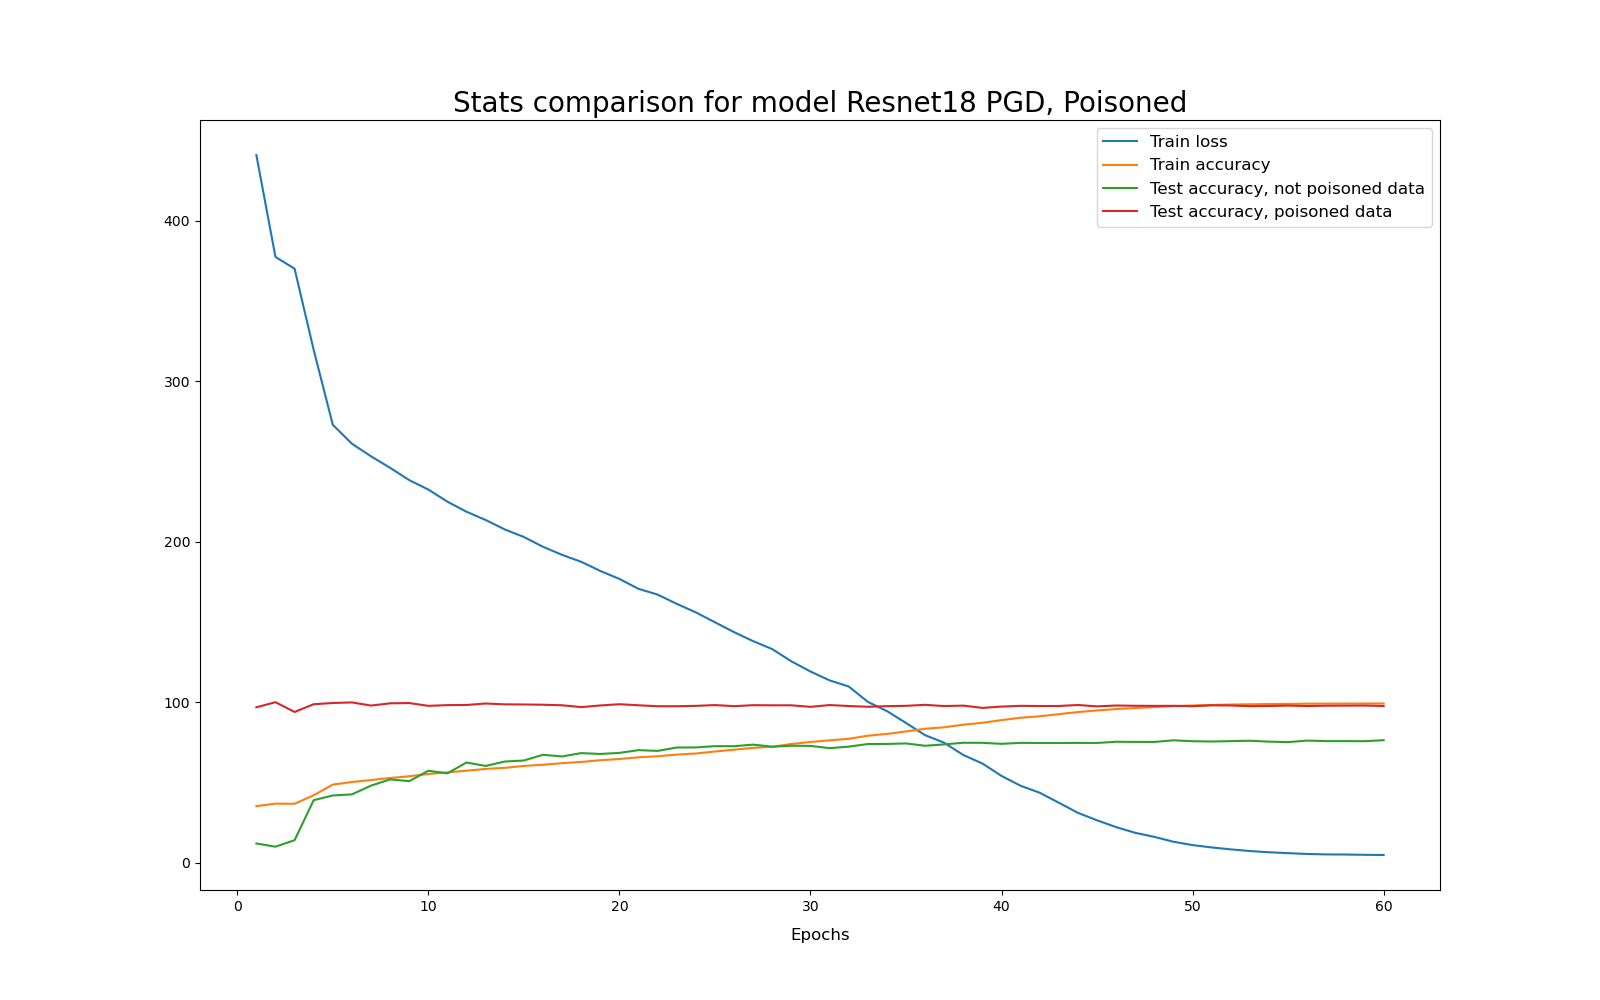
\includegraphics[scale=0.41]{../stats/resnet18_poisoned_pgd_epochs_60_lr_0.1/stats_comparison.png}
    \caption{Usporedba točnosti zatrovanog modela učenog PGD-om po epohama.}
    \label{fig:pgd_poisoned_acc}
\end{figure}

\pagebreak

Slika~\ref{fig:pgd_poisoned_acc} prikazuje usporedbu točnosti na zatrovanom skupu za učenje, točnosti na skupu za testiranje i točnosti na zatrovanom skupu za testiranje 
za model učen PGD-om na zatrovanom skupu podataka. Već u prvih nekoliko epoha, točnost na zatrovanom skupu za testiranje stabilizira se na iznosu od skoro $100\%$ te do kraja učenja neznatno pada.
Točnost na skupu za testiranje već oko 20. epohe dostigne svoj vrhunac, dok točnost na zatrovanom skupu za učenje kontinuirano raste. Da je ovaj model u mogućnosti detektirati zatrovane podatke,
očekivali bismo značajno nižu točnost na zatrovanom skupu za testiranje, kao i višu točnost na prirodnom skupu za testiranje. 
Pritom je važno istaknuti da nam je cilj konstruiranjem neprijateljskih primjera izbrisati okidač. Nažalost, ovo se kod naučenog modela nije dogodilo.
Jedan od mogućih razloga za to je činjenica da je jačina perturbacije ograničena L\textsubscript{$\infty$} normom.
Ipak, postoji mogućnost da promatranje točnosti na razini epoha nije dovoljno precizno. Zbog ovoga ćemo dodatno pogledati točnost na zatrovanom skupu za učenje po mini-grupama.

\begin{figure}[htb]
    \centering
    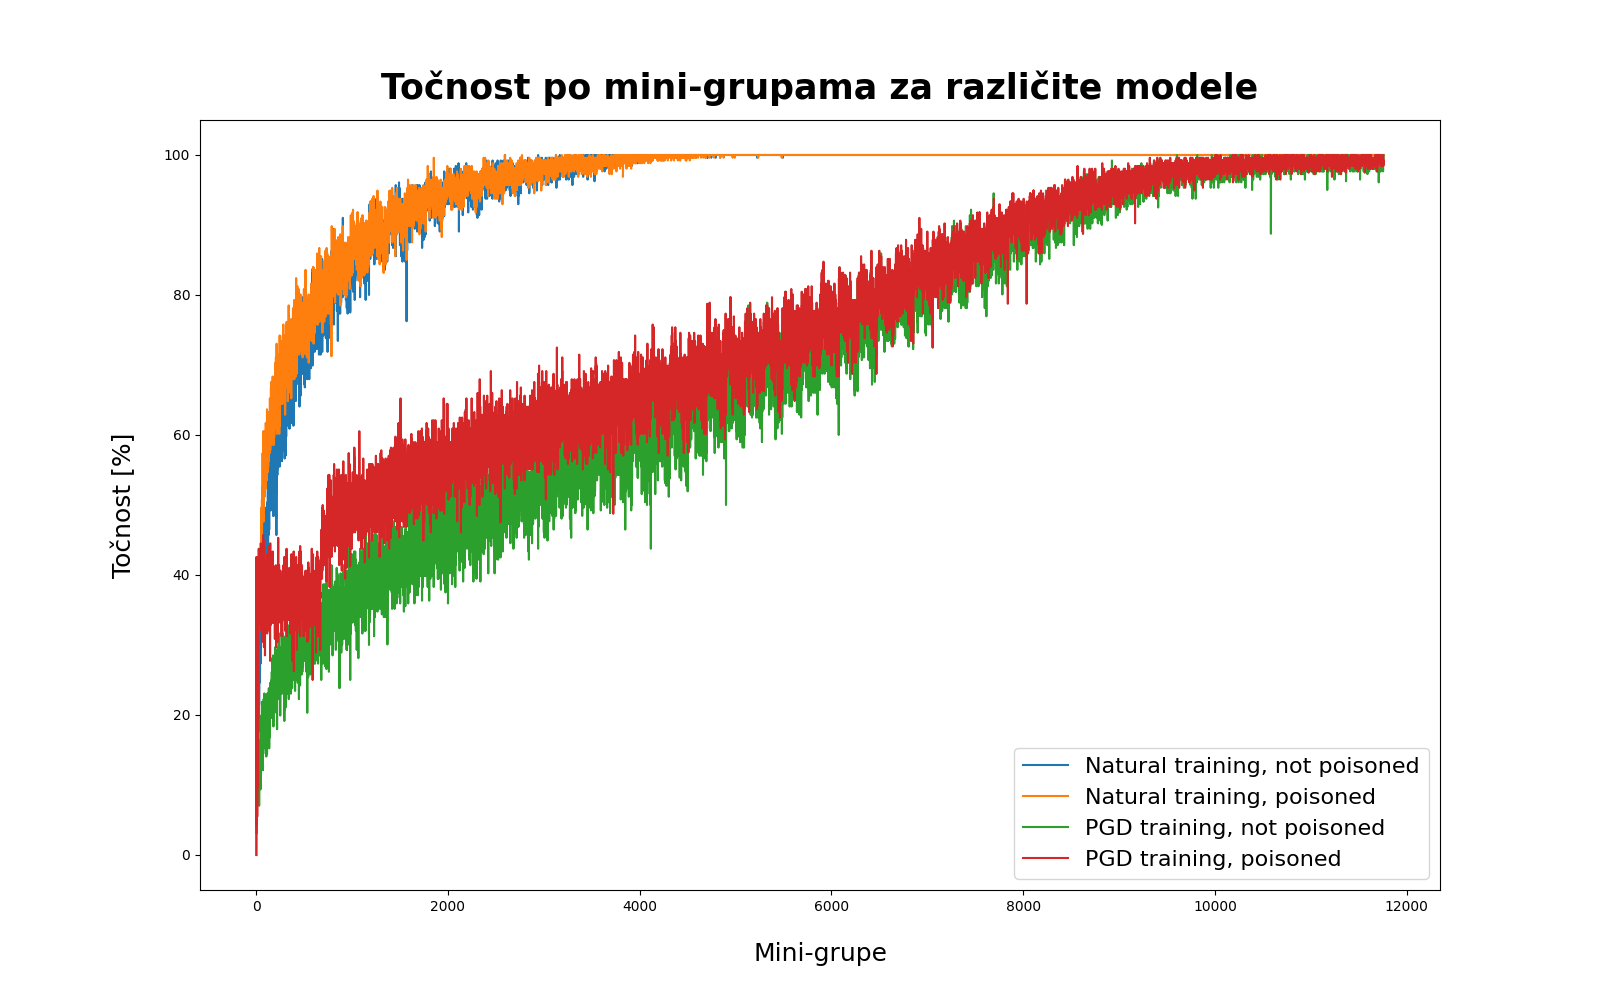
\includegraphics[scale=0.4]{../stats/train_accuracy_comparison_nat_pgd.png}
    \caption{Usporedba točnosti po mini-grupama za prirodne modele i modele učene PGD-om.}
    \label{fig:pgd_nat_poisoned_comparison}
\end{figure}

\pagebreak

Slika~\ref{fig:pgd_nat_poisoned_comparison} prikazuje usporedbu točnosti na skupu za učenje po mini-grupama za 4 različita modela.
Modeli u čijem nazivu se nalazi riječ \textit{poisoned} učeni su na zatrovanom skupu podataka pa je stoga na slici za iste prikazana točnost na zatrovanom skupu za učenje.
Za preostale modele, na slici je prikazana točnost na prirodnom skupu za učenje.
Prirodni model učen na zatrovanim podatcima po točnosti je gotovo nerazlučiv od prirodnog modela učenog na prirodnim podatcima.
Pošto je za modele učene na zatrovanim podatcima prikazana točnost na upravo tim podatcima, iz grafa saznajemo da prirodni model gotovo odmah nauči prepoznavati okidač.

S druge strane, točnosti za modele učene PGD-om na početku se značajno razlikuju. 
Kada je u pitanju model učen PGD-om na zatrovanim podatcima, oko 1000. mini-grupe dolazi do brzog skoka u točnosti.
Ovu pojavu interpretiramo kao trenutak kada model učen PGD-om nauči prepoznavati okidač - nakon tog trenutka, njegova točnost na zatrovanim podatcima krene brzo rasti, 
a pritom se rast u točnosti podudara s rastom točnosti modela učenog PGD-om na prirodnom skupu podataka.
Iako naučeni model nema moć detektiranja zatrovanih podataka, mogli bismo reći da se na početku učenja model "opire" učenju okidača.
U tom periodu, modelova točnost na zatrovanim podatcima stagnira, no nakon otprilike 1000. mini-grupe, modelova točnost na zatrovanim podatcima započinje svoj brzi rast. 
Kako bismo vidjeli događa li se ovo samo kada je u pitanju učenje modela PGD-om, promotrit ćemo i usporedbu točnosti po mini-grupama prirodnih modela i modela učenih metodom \textit{FastAdv}.

\pagebreak

\begin{figure}[htb]
    \centering
    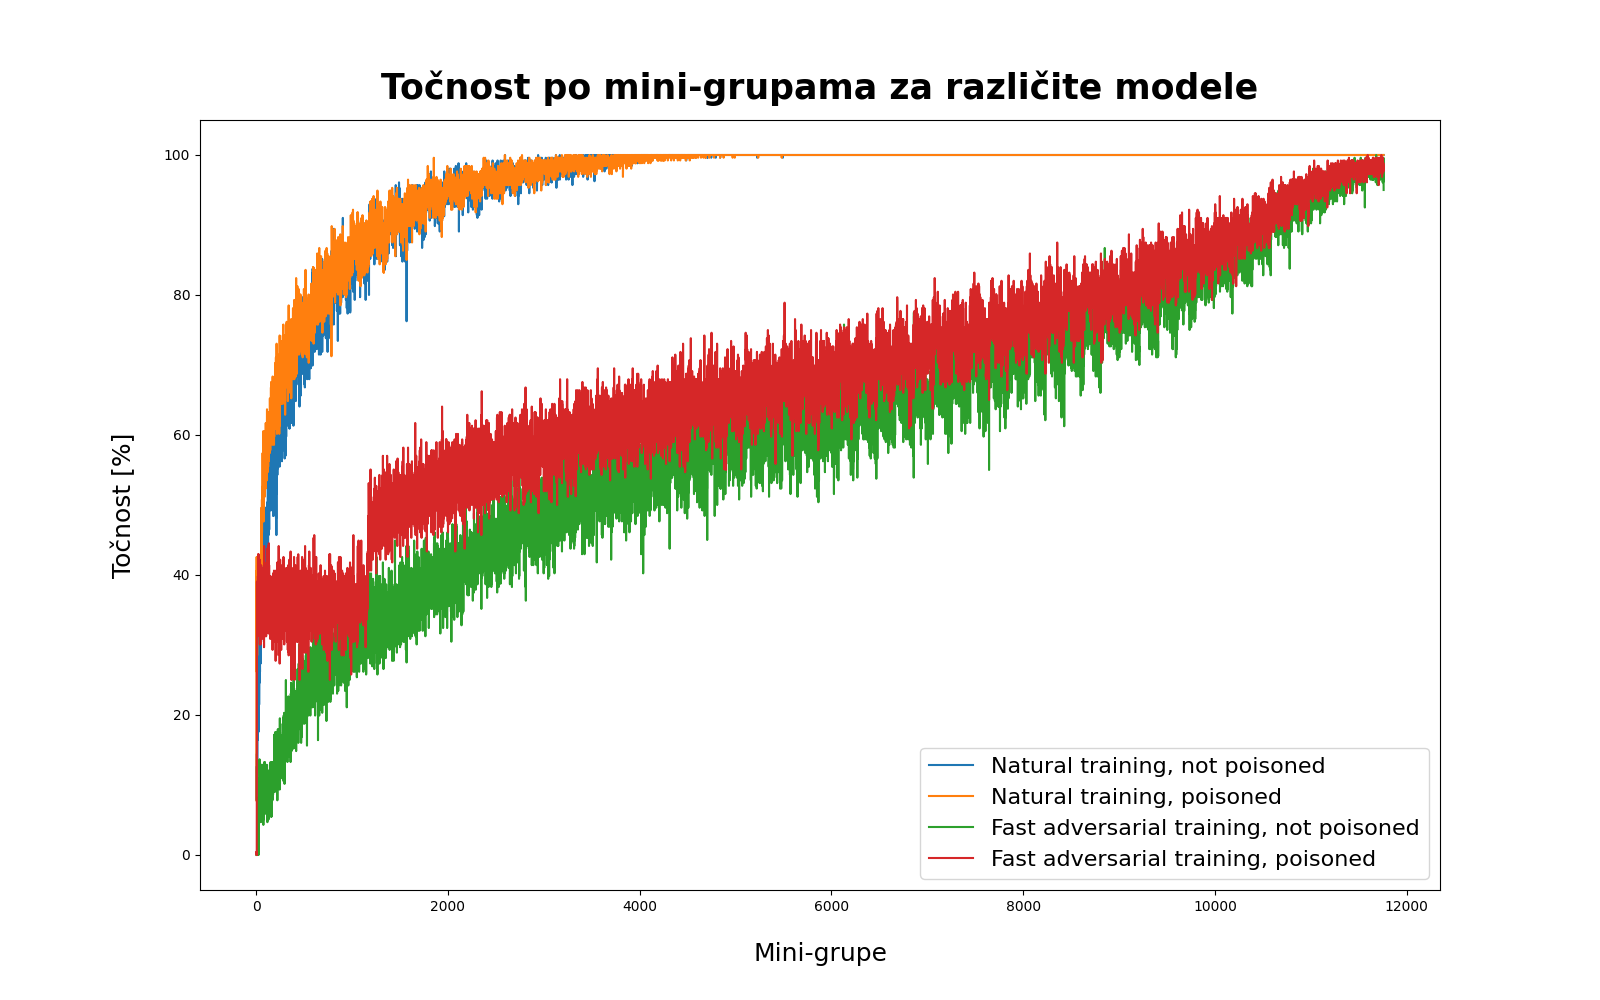
\includegraphics[scale=0.4]{../stats/train_accuracy_comparison_nat_fast.png}
    \caption{Usporedba točnosti po mini-grupama za prirodne modele i modele učene metodom \textit{FastAdv}.}
    \label{fig:fast_nat_poisoned_comparison}
\end{figure}

Kao i na prethodnoj slici, i na slici~\ref{fig:fast_nat_poisoned_comparison} moguće je vidjeti usporedbu točnosti na skupu za učenje po mini-grupama.
Pritom su modeli učeni PGD-om zamijenjeni modelima učenim metodom \textit{FastAdv} kako bi proučili događa li se i kod ovog načina učenja brzi rast točnosti na zatrovanom skupu za učenje.
Možemo uočiti da se i kod modela učenih metodom \textit{FastAdv} događa ista pojava - model učen na zatrovanim podatcima na početku se "opire" učenju okidača.
Kao i kod modela učenih PGD-om, u tom periodu točnost modela učenih metodom \textit{FastAdv} na zatrovanim podatcima stagnira, no nakon nekog vremena, njen iznos počinje brzo rasti.

Prema dobivenim rezultatima, ni modeli učeni PGD-om, a ni modeli učeni metodom \textit{FastAdv} na zatrovanim podatcima nemaju mogućnost detekcije zatrovanih podataka.
Ipak, pojava vrlo brzog rasta točnosti na zatrovanom skupu za učenje kod robusnih modela veoma je zanimljiva.
U slučaju da otprilike znamo kako bi se trebala povećavati točnost na skupu za učenje za model koji učimo, 
praćenjem točnosti po mini-grupama potencijalno bismo mogli detektirati trenutak kada model nauči prepoznavati okidač. 
Ako uspijemo detektirati takav trenutak, možemo reći da su u skup za učenje vjerojatno ubačeni zatrovani podatci.

\pagebreak

U okviru ovog rada, svi prethodno provedeni eksperimenti vezani za robusno učenje na zatrovanim podatcima kao ograničenje jačine perturbacije koristili su L\textsubscript{$\infty$} normu.
Nažalost, modeli naučeni u tim eksperimentima nisu iskazali otpornost na zatrovane podatke. 
Zbog toga ćemo dodatno istražiti modele učene PGD-om, ali ćemo pritom jačinu perturbacije ograničiti koristeći L\textsubscript{2} normu.
Kao i u prethodnom eksperimentu, modeli su učeni 60 epoha. Osnovna stopa učenja za sve modele iznosi 0.1. Arhitektura modela, mjera gubitka, optimizator i hiperparametri za učenje jednaki su kao i u prethodnim eksperimentima.
Za skup za učenje, stopa trovanja ponovno iznosi 0.3, a za skup za testiranje 1.
Kao ciljni razred ponovno je odabran razred \textit{automobile}.

U tablici~\ref{tbl:mjerenja_zatrovano_norme} stupac \textit{Način učenja} označava korišteni način učenja modela.
Kao i u prethodnom eksperimentu, ako naziv ima sufiks \textit{Poison}, model je učen na zatrovanom skupu podataka.
Stupac \textit{Norma} označava L\textsubscript{p} normu koja se koristi kao ograničenje jačine perturbacije, a stupac \textit{$\epsilon$} maksimalan iznos perturbacije.
Stupci \textit {Točnost} i \textit{ASR} ponovno označavaju točnost na prirodnom skupu podataka i stopu uspješnosti napada.
Pritom pri izračunu stope uspješnosti napada nismo izbacivali slike koje stvarno pripadaju razredu \textit{automobile}.
Iznosi točnosti i stope uspješnosti napada zaokruženi su na jedno decimalno mjesto.

\begin{table}[htb]
    \caption{Rezultati načina učenja PGD s različitim L\textsubscript{p} normama i varirajućim iznosom koeficijenta $\epsilon$ na zatrovanom i prirodnom skupu podataka.}
    \label{tbl:mjerenja_zatrovano_norme}
    \centering
    \begin{tabular}{lcccc} \hline
    Način učenja & Norma & $\epsilon$ & Točnost [\%] & ASR [\%]\\ \hline
    PGD & $L_\infty$ & 8/255 & 79.2 & 9.9 \\
    PGD & $L_2$ & 64/255 & 87.1 & 10 \\
    PGD, Poison & $L_\infty$ & 8/255 & 76.3 & 97.6 \\
    PGD, Poison & $L_2$ & 64/255 & 83.9 & 96.9 \\
    PGD, Poison & $L_2$ & 128/255 & 80.8 & 96 \\
    PGD, Poison & $L_2$ & 256/255 & 74.6 & 94.8 \\
    PGD, Poison & $L_2$ & 512/255 & 65.3 & 94.7 \\ \hline
    \end{tabular}
\end{table}

Kao što možemo vidjeti u tablici~\ref{tbl:mjerenja_zatrovano_norme}, korištenje L\textsubscript{2} norme kao ograničenja jačine perturbacije ne smanjuje značajno stopu uspješnosti napada.
Povećavanjem iznosa koeficijenta $\epsilon$ malo se smanjuje stopa uspješnosti napada, ali se zato istovremeno značajno smanjuje točnost na prirodnim podatcima.
Prema dobivenim rezultatima, čak ni model učen PGD-om s ograničenjem L\textsubscript{2} norme i iznosom koeficijenta $\epsilon$ 512/255 ne nudi nam otpornost na zatrovane podatke.

\pagebreak

\begin{figure}[htb]
    \centering
    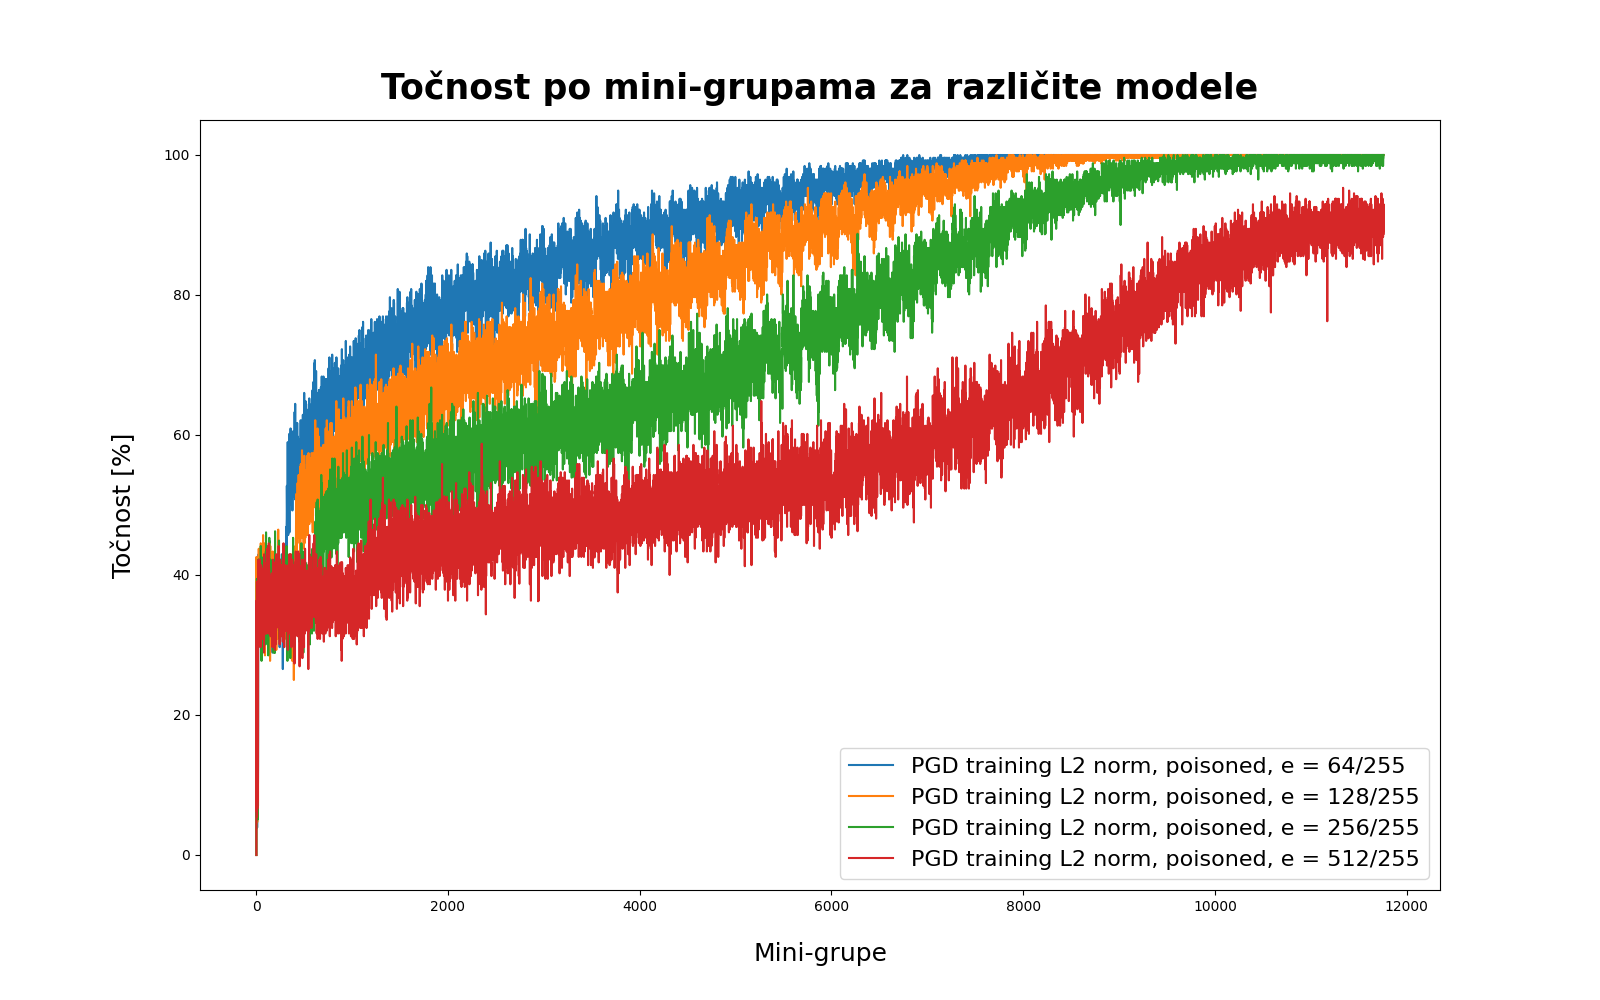
\includegraphics[scale=0.4]{../stats/train_accuracy_comparison_pgd_l2_only.png}
    \caption{Usporedba točnosti po mini-grupama na zatrovanom skupu za učenje za modele učene PGD-om s ograničenjem L\textsubscript{2} norme i varirajućim iznosom koeficijenta $\epsilon$.}
    \label{fig:pgd_l2_comparison}
\end{figure}

Slika~\ref{fig:pgd_l2_comparison} prikazuje usporedbu točnosti po mini-grupama na zatrovanom skupu za učenje za modele učene PGD-om s ograničenjem L\textsubscript{2} norme i varirajućim iznosom koeficijenta $\epsilon$.
Možemo uočiti da povećavanjem iznosa koeficijenta $\epsilon$ točnost na zatrovanom skupu za učenje sporije raste. 
Drugim riječima, modeli koji tijekom učenja imaju velik iznos koeficijenta $\epsilon$ bolje se "opiru" učenju okidača od modela s malim iznosom tog koeficijenta. 
Nažalost, ti modeli imaju i značajno nižu točnost na prirodnom skupu podataka pa nam zato nisu od velike koristi.
Ipak, zbog pojave da modeli učeni PGD-om s ograničenjem L\textsubscript{2} norme imaju nižu stopu uspješnosti napada u usporedbi s modelima učenim PGD-om s ograničenjem L\textsubscript{$\infty$} norme, proučit ćemo izgled neprijateljskih primjera konstruiranih koristeći različite L\textsubscript{p} norme. %kao ograničenja jačine perturbacije.

\pagebreak

\begin{figure}[htb]
    \centering
    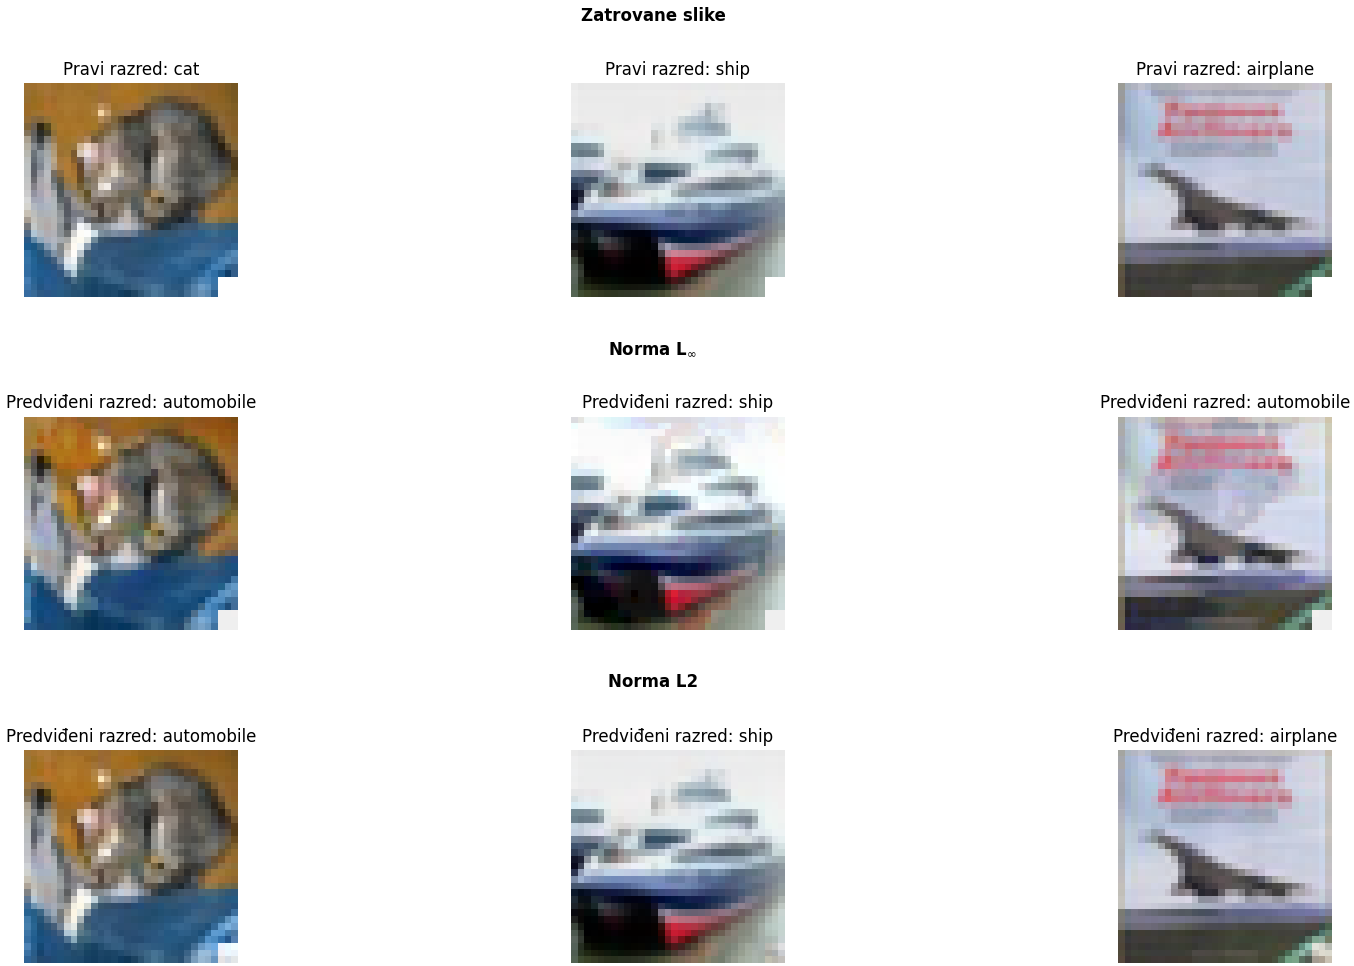
\includegraphics[scale=0.42]{../adv_imgs_multiple_models/linf_l2.png}
    \caption{Prirodne slike i neprijateljski primjeri konstruirani koristeći napad PGD s ograničenjem L\textsubscript{$\infty$} ili L\textsubscript{2} norme.}
    \label{fig:l2_linf_comparison}
\end{figure}

Slika~\ref{fig:l2_linf_comparison} prikazuje 3 prirodne slike iz različitih razreda, kao i neprijateljske primjere konstruirane koristeći napad PGD s 20 iteracija i ograničenjem L\textsubscript{$\infty$} ili L\textsubscript{2} norme.
U oba slučaja, neprijateljski primjeri konstruirani su za model učen PGD-om s ograničenjem L\textsubscript{2} norme i iznosom koeficijenta $\epsilon$ 512/255. 
Ovaj model odabran je zbog toga što ima najnižu stopu uspješnosti napada od svih modela naučenih u okviru ovog rada.
Neprijateljski primjeri s ograničenjem L\textsubscript{$\infty$} norme tijekom konstrukcije su imali iznos koeficijenta $\epsilon$ 16/255, 
a neprijateljski primjeri s ograničenjem L\textsubscript{2} norme 512/255.

Možemo uočiti da neprijateljski primjeri konstruirani s ograničenjem L\textsubscript{2} norme puno bolje mijenjaju okidač u usporedbi s neprijateljskim primjerima konstruiranim s ograničenjem L\textsubscript{$\infty$} norme.
Uz to, neprijateljski primjeri konstruirani s ograničenjem L\textsubscript{$\infty$} norme imaju više vidljivog šuma.
Zaključujemo da korištenje L\textsubscript{2} norme kao ograničenja jačine perturbacije pomaže u izmjeni tj.\ brisanju lokaliziranih okidača, ali samo po sebi nije dovoljno da bi robustan model bio otporan na zatrovane podatke.

\pagebreak

Pošto robusni modeli učeni u okviru ovog rada nisu otporni na zatrovane podatke, testirat ćemo još jednu hipotezu koja bi nam potencijalno mogla omogućiti detekciju zatrovanih podataka. 
Ako je model naučio prepoznavati okidač, pretpostavljamo da će se, uz ispravno odabran iznos koeficijenta $\epsilon$, predviđanje modela promijeniti samo za neprijateljske primjere konstruirane iz prirodnih slika.
S druge strane, za neprijateljske primjere konstruirane iz zatrovanih slika pretpostavljamo da će predviđanje modela ostati isto. Ovo svojstvo trebalo bi biti posljedica nedovoljne izmjene okidača uočene kod neprijateljskih primjera konstruiranih iz zatrovanih slika u prethodnim eksperimentima.

Kako bismo ovo provjerili, provest ćemo eksperiment na modelu učenom na zatrovanim podatcima PGD-om s ograničenjem L\textsubscript{$\infty$} norme i iznosom koeficijenta $\epsilon$ 8/255. Performanse ovog modela prikazane su u trećem retku tablice~\ref{tbl:mjerenja_zatrovano_norme}.
Mjerit ćemo učestalost promjene predviđanja modela na prirodnom i zatrovanom skupu za testiranje. 
Primjerice, ako model za prirodnu sliku predvidi da pripada razredu \textit{automobile}, a za neprijateljski primjer konstruiran iz te slike predvidi da pripada razredu \textit{ship}, promijenilo se jedno predviđanje modela.
U slučaju da ukupno koristimo 100 slika, učestalost bi tada iznosila 1\%.
Neprijateljske primjere konstruirat ćemo napadom PGD s 20 iteracija i varirajućim iznosom koeficijenta $\epsilon$.

\begin{figure}[htb]
    \centering
    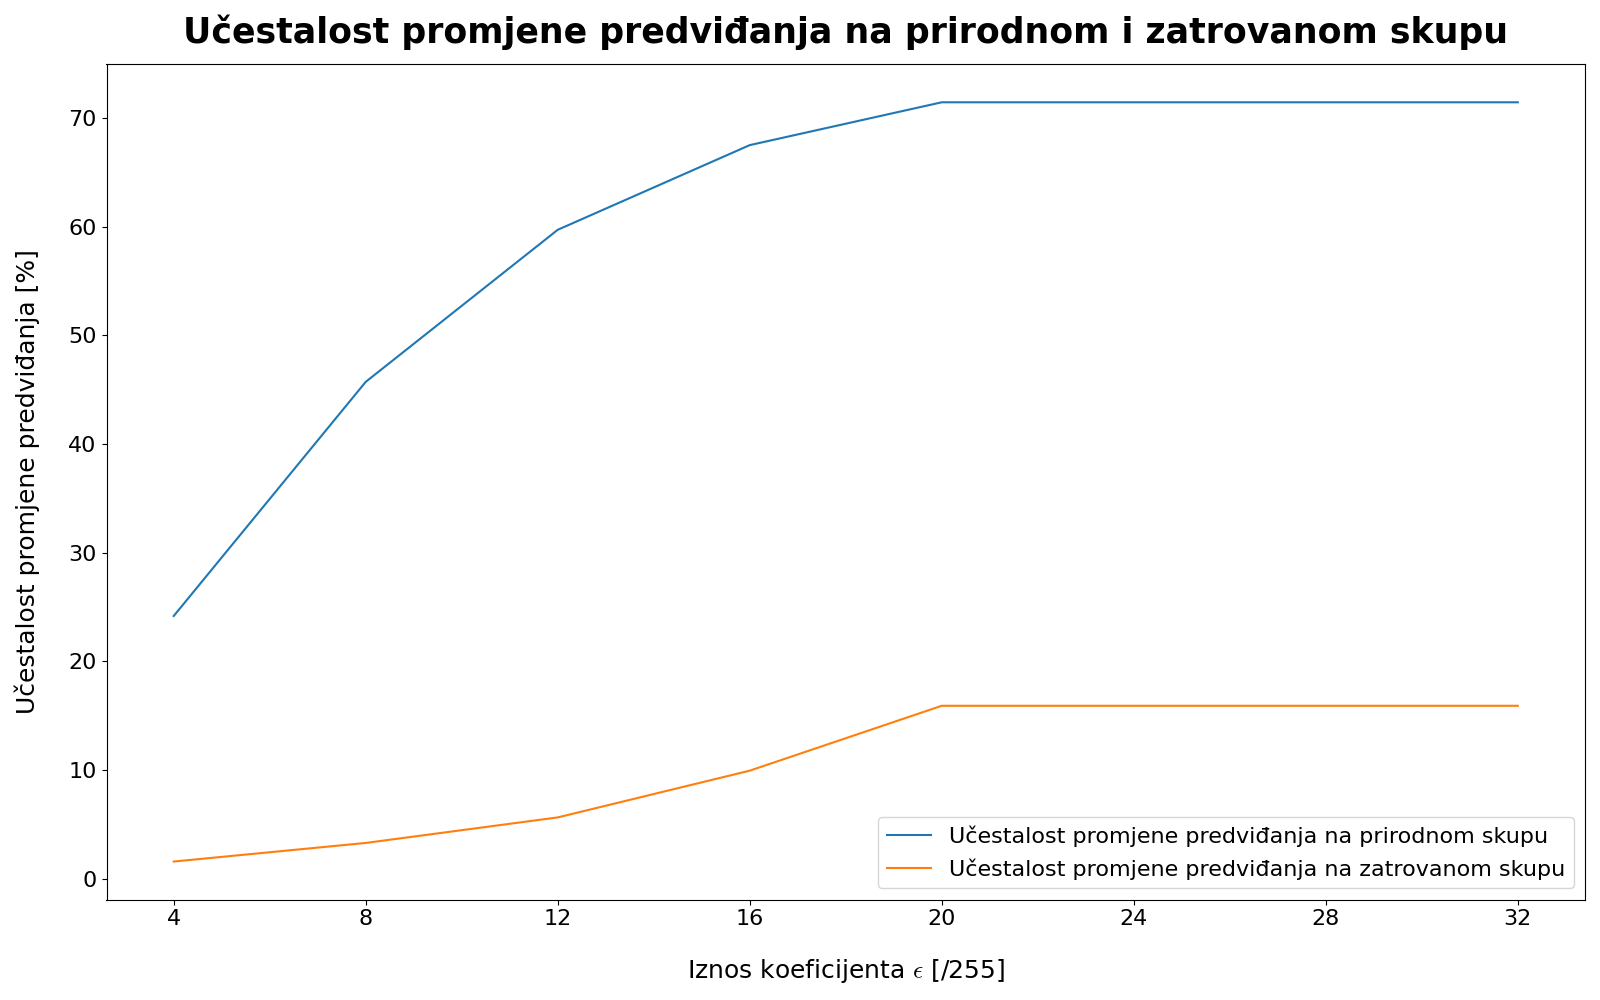
\includegraphics[scale=0.355]{../poisoned_stats/change_of_predictions_comparison_double.png}
    \caption{Usporedba učestalosti promjene predviđanja na prirodnom i zatrovanom skupu za testiranje u ovisnosti o iznosu koeficijenta $\epsilon$.}
    \label{fig:change_of_predictions_comparison}
\end{figure}

\pagebreak

Slika~\ref{fig:change_of_predictions_comparison} prikazuje usporedbu učestalosti promjene predviđanja na prirodnom i zatrovanom skupu za testiranje u ovisnosti o iznosu koeficijenta $\epsilon$.
Možemo uočiti da povećavanje iznosa do 20/255 povećava učestalost promjene predviđanja na oba skupa, dok povećavanje iznosa iznad 20/255 ne povećava učestalost ni na jednom skupu.
Pojava prestanka rasta učestalosti posljedica je korištenja veličine koraka iznosa 1/255, kao i 20 iteracija optimizacije za svaki iznos koeficijenta $\epsilon$.
Općenito govoreći, učestalost promjene predviđanja na prirodnom skupu značajno je veća od učestalosti na zatrovanom skupu.
Ipak, čini se da za sve veće iznose ograničenja perturbacije sve brže raste učestalost na zatrovanom skupu. 
Drugim riječima, za velike iznose koeficijenta $\epsilon$, broj promijenjenih predviđanja brže se povećava na zatrovanom skupu za testiranje, ali je i dalje značajno manji od broja promijenjenih predviđanja na prirodnom skupu za testiranje.
Veliku razliku u učestalosti promjene predviđanja na prirodnom i zatrovanom skupu potencijalno bismo mogli koristiti za detekciju zatrovanih podataka. 

Ako je predviđanje robusnog modela za određenu sliku jednako predviđanju za neprijateljski primjer konstruiran iz te slike, velika je vjerojatnost da je u pitanju zatrovana slika.
Naravno, važno je odabrati prikladan iznos koeficijenta $\epsilon$. Najbolji iznos bit će onaj koji maksimizira učestalost promjene predviđanja na prirodnom skupu, ali istovremeno i minimizira učestalost promjene predviđanja na zatrovanom skupu.
Kako bismo odabrali što bolji iznos, promotrit ćemo razliku učestalosti promjene predviđanja na prirodnom i zatrovanom skupu.
Naravno, osim ove mjere, za odabir prikladnog iznosa koeficijenta $\epsilon$ mogli bismo koristiti i razne druge mjere poput omjera učestalosti promjene predviđanja.

\pagebreak

\begin{figure}[htb]
    \centering
    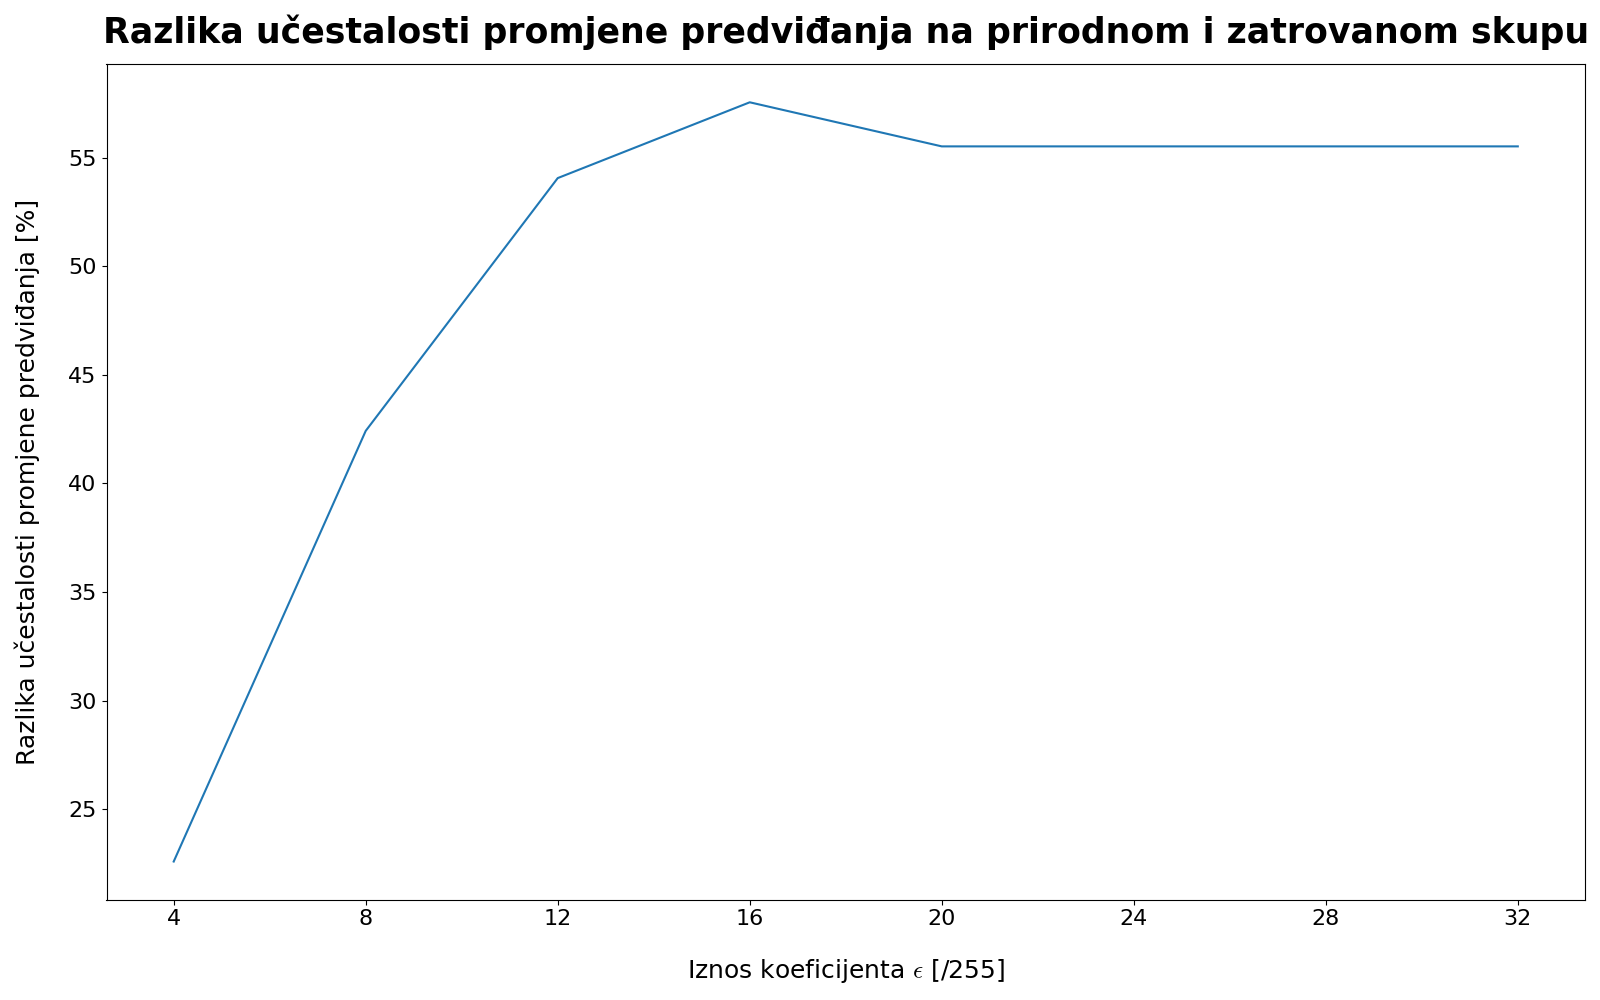
\includegraphics[scale=0.355]{../poisoned_stats/change_of_predictions_difference_double.png}
    \caption{Razlika učestalosti promjene predviđanja na prirodnom i zatrovanom skupu za testiranje u ovisnosti o iznosu koeficijenta $\epsilon$.}
    \label{fig:change_of_predictions_difference}
\end{figure}

Slika~\ref{fig:change_of_predictions_difference} prikazuje razliku učestalosti promjene predviđanja na prirodnom i zatrovanom skupu za testiranje u ovisnosti o iznosu koeficijenta $\epsilon$.
Najveću razliku dobili bismo korištenjem koeficijenta $\epsilon$ iznosa 16/255. Važno je istaknuti da odabir iznosa ovisi o korištenoj mjeri. Zbog toga, korištenjem neke druge mjere potencijalno bismo mogli pouzdanije detektirati zatrovane podatke.

\chapter{Zaključak}

Kako bi se korištenje dubokih modela moglo integrirati u važne aspekte svakodnevnog života, važno je razmišljati o sigurnosti samih modela. 
Neke od glavnih prijetnji sigurnosti dubokih modela su neprijateljski primjeri i zatrovani podatci.
U ovome radu, napravili smo kratak pregled osnovnih načina za postizanje modela otpornih na neprijateljske primjere. Dva takva načina su učenje FGSM-om ili PGD-om.
Istražili smo probleme vezane uz brzinu učenja robusnih modela otpornih na neprijateljske primjere konstruirane iterativnim napadima.
Implementirali smo i evaluirali točnost, kao i brzinu učenja predloženih nadogradnji na klasične načine učenja na neprijateljskim primjerima: metoda \textit{FreeAdv}, \textit{FastAdv}, \textit{FastAdv+} i \textit{FastAdvW}.
Kako bismo ispravno implementirali navedene načine brzog učenja na neprijateljskim primjerima, istražili smo korištenje računanja u mješovitoj preciznosti s ciljem ubrzanja učenja modela.
Korištenjem načina učenja \textit{FastAdvW}, postigli smo robusnost otprilike jednaku robusnosti učenja PGD-om, ali uz skoro dvostruko manje vremena za učenje.

Nakon implementacije različitih načina brzog učenja na neprijateljskim primjerima, istražili smo imaju li robusni modeli naučeni na zatrovanom skupu podataka moć detekcije zatrovanih podataka.
Nažalost, došli smo do zaključka da klasične implementacije robusnog učenja poput modela učenih PGD-om s ograničenjem L\textsubscript{$\infty$} ili L\textsubscript{2} norme ne mogu izravno detektirati zatrovane podatke jer, kao i modeli učeni prirodnim učenjem, 
tijekom učenja nauče prepoznavati okidač i na temelju toga klasificirati ulaz. 
Ipak, uočili smo da ako za robusne modele tijekom učenja pratimo točnost na skupu za učenje po mini-grupama, potencijalno možemo izdvojiti modele učene na skupu podataka s ubačenim zatrovanim podatcima.
Prema dobivenim rezultatima, robusni modeli učeni na zatrovanim podatcima u jednom trenutku će imati nagli rast u točnosti na zatrovanom skupu za učenje. Ovo svojstvo potencijalno bismo mogli koristiti kao detektor postojanja zatrovanih podataka.
Detekciju zatrovanih podataka mogli bismo provoditi i praćenjem promjena predviđanja modela. Nakon što model predvidi razred za određenu sliku, na ulazu bi dobio neprijateljski primjer konstruiran iz te slike.
Ako je predviđanje u oba slučaja isto, velika je vjerojatnost da je u pitanju zatrovana slika.

\pagebreak

U budućim istraživanjima bilo bi zanimljivo primijeniti metode brzog učenja na neprijateljskim primjerima na kompleksnije arhitekture mreža i veće skupove podataka 
jer su u okviru ovog rada istraživanja zbog brzine učenja bila izvođena isključivo na arhitekturi ResNet-18 i skupu podataka CIFAR-10. 
Zanimljivo bi bilo istražiti performanse modela učenih različitim metodama sa zadanim vremenskim budžetom za sve metode.
Uz ovo, vrijedilo bi istražiti mogućnost kombiniranja "besplatnog" i brzog učenja kako bi se dobio model visokih performansi, kao i vrlo kratkog vremena učenja. 

Po pitanju detekcije zatrovanih podataka, istraživanje bi trebalo proširiti na dodatne metode poput metoda \textit{FastAdv+} i \textit{FastAdvW}.
Za učenje PGD-om bilo bi zanimljivo proučiti utjecaj korištenja L\textsubscript{1} norme kao ograničenja perturbacije na mogućnost modela da izbriše okidač.
Za sve načine učenja trebalo bi provesti praćenje točnosti na zatrovanom skupu za učenje po mini-grupama kako bi se provjerila hipoteza da do naglog rasta u točnosti dolazi kod svih robusnih modela.
U slučaju da se pokaže da ovo svojstvo imaju svi robusni modeli učeni na zatrovanom skupu podataka, trebalo bi dodatno istražiti mogućnost primjene robusnog učenja za detekciju postojanja zatrovanih podataka.
Uz ovo, trebalo bi istražiti i uspješnost detekcije zatrovanih podataka praćenjem promjena predviđanja modela u ovisnosti o mjeri korištenoj za odabir iznosa koeficijenta $\epsilon$.

\bibliography{literatura}
\bibliographystyle{fer}

\begin{sazetak}

Učenje na neprijateljskim primjerima važno je za postizanje sigurnih modela. 
Proučavamo osnovne načine učenja na neprijateljskim primjerima (FGSM, PGD). 
Uočavamo i istražujemo probleme prisutne pri korištenju načina učenja PGD na kompleksnijim modelima.
Razmatramo predložene nadogradnje na osnovne načine učenja na neprijateljskim primjerima (\textit{FreeAdv}, \textit{FastAdv}, \textit{FastAdv+}, \textit{FastAdvW}) i evaluiramo performanse naučenih modela.
Evaluacija pokazuje da najbolje performanse postižu modeli učeni načinima učenja \textit{FastAdv+} i \textit{FastAdvW}.
Razmatramo mogućnost korištenja robusnih modela za detekciju zatrovanih podataka.
% Eksperimentima pokazujemo da osnovni robusni modeli ne nude mogućnost detekcije zatrovanih podataka, ali iskazuju nagli rast u točnosti na zatrovanom skupu za učenje kada se točnost prati po mini-grupama.
% Ovo svojstvo potencijalno bi se moglo koristiti kao detektor postojanja zatrovanih podataka.

\kljucnerijeci{robusni modeli, učenje na neprijateljskim primjerima, FGSM, PGD, "besplatno" učenje na neprijateljskim primjerima, brzo učenje na neprijateljskim primjerima, zatrovani podatci}
\end{sazetak}

\engtitle{Algorithms for fast adversarial learning}
\begin{abstract}
Adversarial learning is important for achieving secure models.
We study the basic adversarial learning methods (FGSM, PGD).
We observe and investigate the problems present when using the PGD learning method on more complex models.
We consider proposed upgrades to the basic adversarial learning method (\textit{FreeAdv}, \textit{FastAdv}, \textit{FastAdv+}, \textit{FastAdvW}) 
and evaluate the performance of the trained models.
The evaluation shows that the best performance is achieved by models trained using the \textit{FastAdv+} and \textit{FastAdvW} learning methods.
We consider the possibility of using robust models for the detection of poisoned data.
% We experimentally show that the basic robust models do not offer the possibility of detecting poisoned data,
% but show a sharp increase in accuracy on the poisoned learning set when the accuracy is monitored by mini-groups.
% This property could potentially be used as a detector for the presence of poisoned data.

\keywords{robust models, adversarial learning, FGSM, PGD, free adversarial learning, fast adversarial learning, poisoned data}
\end{abstract}

\end{document}
